% Para utilizar este template siga o tutorial disponível em http://www.biblioteca.ufc.br/images/arquivos/instrucoes_modelos/tutorial_sharelatex.pdf

%%%%%%%%%%%%%%%%%%%%%%%%%%%%%%%%%%%%%%%%%%%%%%%%%%%%%%%
%% Você deve criar uma conta no ShareLatex. Depois,  %%
%% vá nas opções no canto esquerdo superior da tela  %%
%% e clique em "Copiar Projeto". Dê um novo nome pa- %%
%% ra o projeto.                                     %%
%%                                                   %%
%% Os principais desenvolvedores deste template são: %%
%%                                                   %%
%%            Ednardo Moreira Rodrigues              %%
%%     (Doutorando em Engenharia Elétrica - UFC)     %%
%%                      &                            %%
%%            Alan Batista de Oliveira               %%
%%     (Graduando em Engenharia Elétrica - UFC)      %%
%%                                                   %%
%% Revisão:                                          %%
%%                                                   %%
%% - Eliene Maria Vieira de Moura;                   %%
%% - Francisco Edvander Pires Santos;                %%
%% - Izabel Lima dos Santos;                         %%
%% - Juliana Soares Lima;                            %%
%% - Kalline Yasmin Soares Feitosa.                  %%
%%                                                   %%
%% Colaboradores                                     %%
%%                                                   %%
%% -Andrei Bosco Bezerra Torres                      %% 
%% (Professor - Sistemas e Mídias Digitais -         %%
%% Instituto Universidade Virtual - UFC)             %%
%% Tiago ALves Lima                                  %% 
%% (Aluno de Mestrado em Eng. Elétrica)              %%
%%                                                   %%
%% Grande parte do trabalho foi adaptado do template %%
%% da UECE elaborado por:                            %%
%% Thiago Nascimento  (UECE)                         %%
%% Project available on:                             %%
%% https://github.com/thiagodnf/uecetex2             %%
%%                                                   %%
%% "Dúvidas, esclarecimentos ou sugestões podem ser  %%
%% enviadas para o e-mail da Comissão de Serviços da %%
%% Biblioteca Universitária:                         %%
%%          bu@ufc.br ou bchleitor@ufc.br"           %%
%%                                                   %%
%% As últimas atualizações estão descritas no inicio %%
%% do arquivo "README.md".                           %%
%%                                                   %%
%%%%%%%%%%%%%%%%%%%%%%%%%%%%%%%%%%%%%%%%%%%%%%%%%%%%%%%

\documentclass[        
    a4paper,          % Tamanho da folha A4
    12pt,             % Tamanho da fonte 12pt
    chapter=TITLE,    % Todos os capitulos devem ter caixa alta
    section=Title,    % Todas as secoes devem ter caixa alta somente na primeira letra
    subsection=Title, % Todas as subsecoes devem ter caixa alta somente na primeira letra
    oneside,          % Usada para impressao em apenas uma face do papel
    english,          % Hifenizacoes em ingles
    spanish,          % Hifenizacoes em espanhol
    brazil,           % Ultimo idioma eh o idioma padrao do documento
    fleqn             % Coloca as equações alinhadas a esquerda
]{abntex2}


% Para utilizar este template siga o tutorial disponível em http://www.biblioteca.ufc.br/images/arquivos/instrucoes_modelos/tutorial_sharelatex.pdf

%%%%%%%%%%%%%%%%%%%%%%%%%%%%%%%%%%%%%%%%%%%%%%%%%%%%%%%
%% Você deve criar uma conta no ShareLatex. Depois,  %%
%% vá nas opções no canto esquerdo superior da tela  %%
%% e clique em "Copiar Projeto". Dê um novo nome pa- %%
%% ra o projeto.                                     %%
%%                                                   %%
%% Os principais desenvolvedores deste template são: %%
%%                                                   %%
%%            Ednardo Moreira Rodrigues              %%
%%     (Doutorando em Engenharia Elétrica - UFC)     %%
%%                      &                            %%
%%            Alan Batista de Oliveira               %%
%%     (Graduando em Engenharia Elétrica - UFC)      %%
%%                                                   %%
%% Revisão:                                          %%
%%                                                   %%
%% - Eliene Maria Vieira de Moura;                   %%
%% - Francisco Edvander Pires Santos;                %%
%% - Izabel Lima dos Santos;                         %%
%% - Juliana Soares Lima;                            %%
%% - Kalline Yasmin Soares Feitosa.                  %%
%%                                                   %%
%% Colaboradores                                     %%
%%                                                   %%
%% -Andrei Bosco Bezerra Torres                      %% 
%% (Professor - Sistemas e Mídias Digitais -         %%
%% Instituto Universidade Virtual - UFC)             %%
%% Tiago ALves Lima                                  %% 
%% (Aluno de Mestrado em Eng. Elétrica)              %%
%%                                                   %%
%% Grande parte do trabalho foi adaptado do template %%
%% da UECE elaborado por:                            %%
%% Thiago Nascimento  (UECE)                         %%
%% Project available on:                             %%
%% https://github.com/thiagodnf/uecetex2             %%
%%                                                   %%
%% "Dúvidas, esclarecimentos ou sugestões podem ser  %%
%% enviadas para o e-mail da Comissão de Serviços da %%
%% Biblioteca Universitária:                         %%
%%          bu@ufc.br ou bchleitor@ufc.br"           %%
%%                                                   %%
%% As últimas atualizações estão descritas no inicio %%
%% do arquivo "README.md".                           %%
%%                                                   %%
%%%%%%%%%%%%%%%%%%%%%%%%%%%%%%%%%%%%%%%%%%%%%%%%%%%%%%%

% Importações de pacotes
\usepackage[utf8]{inputenc}                         % Acentuação direta
\usepackage[T1]{fontenc}                            % Codificação da fonte em 8 bits
\usepackage{graphicx}                               % Inserir figuras
\usepackage{amsfonts, amssymb, amsmath}             % Fonte e símbolos matemáticos
\usepackage{booktabs}                               % Comandos para tabelas
\usepackage{verbatim}                               % Texto é interpretado como escrito no documento
\usepackage{multirow, array}                        % Múltiplas linhas e colunas em tabelas
\usepackage{indentfirst}                            % Endenta o primeiro parágrafo de cada seção.
\usepackage{listings}                               % Utilizar codigo fonte no documento
\usepackage{xcolor}
\usepackage{microtype}                              % Para melhorias de justificação?
\usepackage[portuguese,ruled,lined]{algorithm2e}    % Escrever algoritmos
\usepackage{algorithmic}                            % Criar Algoritmos  
%\usepackage{float}                                 % Utilizado para criação de floats
\usepackage{amsgen}
\usepackage{lipsum}                                 % Usar a simulação de texto Lorem Ipsum
%\usepackage{titlesec}                              % Permite alterar os títulos do documento
\usepackage{tocloft}                                % Permite alterar a formatação do Sumário
\usepackage{etoolbox}                               % Usado para alterar a fonte da Section no Sumário
\usepackage[nogroupskip,nonumberlist]{glossaries}   % Permite fazer o glossario

\usepackage[font=singlespacing,format=plain,justification=justified,skip=0pt,singlelinecheck = false]{caption}            % Altera o comportamento da tag caption

\usepackage[alf, abnt-emphasize=bf, recuo=0cm, abnt-etal-cite=2, abnt-etal-list=0, abnt-etal-text=it]{abntex2cite}  % Citações padrão ABNT
%\usepackage[bottom]{footmisc}                      % Mantém as notas de rodapé sempre na mesma posição
%\usepackage{times}                                 % Usa a fonte Times
%%%%%%%%%%%%%%%%%%% AVISO %%%%%%%%%%%%%%%%%%%%%%%%%%%%%%%%%%%%%%%%
%descomente as duas linhas abaixo para alterar o texto de Times New Roman para Arial:

%\usepackage{helvet}
%\renewcommand{\familydefault}{\sfdefault}  % Usa a fonte Arial              
%%%%%%%%%%%%%%%%%%%%%%%%%%%%%%%%%%%%%%%%%%%%%%%%%%%%%%%%%%%%%%%%%%

\usepackage{mathptmx}         % Usa a fonte Times New Roman			%\usepackage{lmodern}         % Usa a fonte Latin Modern
%\usepackage{subfig}          % Posicionamento de figuras
%\usepackage{scalefnt}        % Permite redimensionar tamanho da fonte
%\usepackage{color, colortbl} % Comandos de cores
%\usepackage{lscape}          % Permite páginas em modo "paisagem"
%\usepackage{ae, aecompl}     % Fontes de alta qualidade
%\usepackage{picinpar}        % Dispor imagens em parágrafos
%\usepackage{latexsym}        % Símbolos matemáticos
%\usepackage{upgreek}         % Fonte letras gregas
\usepackage{appendix}         % Gerar o apendice no final do documento
\usepackage{paracol}          % Criar paragrafos sem identacao
\usepackage{lib/ufctex}	      % Biblioteca com as normas da UFC para trabalhos academicos
\usepackage{pdfpages}         % Incluir pdf no documento
\usepackage{amsmath}          % Usar equacoes matematicas

\makeglossaries % Organiza e gera a lista de abreviaturas, simbolos e glossario
\makeindex      % Gera o Indice do documento         

\setlength{\mathindent}{0pt} %Complementa o alinhamento de equações para totalmente a esquerda.


%%%%%%%%%%%%%%%%%%%%%%%%%%%%%%%%%%%%%%%%%%%%%%%%%%%%%
%%                     ATENCAO                     %%
%%%%%%%%%%%%%%%%%%%%%%%%%%%%%%%%%%%%%%%%%%%%%%%%%%%%%
%  Qual e o nivel do trabalho academico que voce esta 
% escrevendo? Retire o simbolo "%" apenas de um dos 
% quatro topicos abaixo refente ao nível do seu traba
% -lho.

\trabalhoacademico{tccgraduacao}
%\trabalhoacademico{tccespecializacao}
%\trabalhoacademico{dissertacao}
%\trabalhoacademico{tese}

%%%%%%%%%%%%%%%%%%%%%%%%%%%%%%%%%%%%%%%%%%%%%%%%%%%%%

% Define se o trabalho e uma qualificacao
% Coloque 'nao' para versao final do trabalho

\ehqualificacao{nao}

% Remove as bordas vermelhas e verdes do PDF gerado
% Coloque 'sim' pare remover

\removerbordasdohyperlink{sim} 

% Adiciona a cor Azul a todos os hyperlinks

\cordohyperlink{nao}

%%%%%%%%%%%%%%%%%%%%%%%%%%%%%%%%%%%%%%%%%%%%%%%%%%%%%
%%         Informacao sobre a instituicao          %%
%%%%%%%%%%%%%%%%%%%%%%%%%%%%%%%%%%%%%%%%%%%%%%%%%%%%%

\ies{Universidade Federal do Ceará}
\iessigla{UFC}
\centro{Campus de Quixadá}
%\departamento{Departamento de Xxxxxxxxx}

%%%%%%%%%%%%%%%%%%%%%%%%%%%%%%%%%%%%%%%%%%%%%%%%%%%%%
%%        Informacao para TCC de Graduacao         %%
%%%%%%%%%%%%%%%%%%%%%%%%%%%%%%%%%%%%%%%%%%%%%%%%%%%%%

\graduacaoem{Engenharia de Software}
\habilitacao{bacharel} % Ou licenciado(a)

% AVISO: Caso necessario alterar o texto de apresenta-
% cao da Especializacao ir a pasta "lib", arquivo 
% "ufctex.sty" na linha 502.


%%%%%%%%%%%%%%%%%%%%%%%%%%%%%%%%%%%%%%%%%%%%%%%%%%%%%
%%     Informacao para TCC de Especializacao       %%
%%%%%%%%%%%%%%%%%%%%%%%%%%%%%%%%%%%%%%%%%%%%%%%%%%%%%

\especializacaoem{Yyyyyyyyy}

% AVISO: Caso necessario alterar o texto de apresenta-
% cao da Especializacao, ir a pasta "lib", arquivo 
% "ufctex.sty" na linha 507.

%%%%%%%%%%%%%%%%%%%%%%%%%%%%%%%%%%%%%%%%%%%%%%%%%%%%%
%%         Informacao para Dissertacao             %%
%%%%%%%%%%%%%%%%%%%%%%%%%%%%%%%%%%%%%%%%%%%%%%%%%%%%%

\programamestrado{Programa de Pós-Graduação em Xxxxxxx}
\nomedomestrado{Mestrado Acadêmico em Xxxxxxx}
\mestreem{Engenharia Xxxxxx}
\areadeconcentracaomestrado{Engenharia Xxxxxx}

% AVISO: Caso necessario alterar o texto de apresenta-
% cao da dissertacao, ir a pasta "lib", arquivo 
% "ufctex.sty" na linha 511.

%%%%%%%%%%%%%%%%%%%%%%%%%%%%%%%%%%%%%%%%%%%%%%%%%%%%%
%%               Informação para Tese              %%
%%%%%%%%%%%%%%%%%%%%%%%%%%%%%%%%%%%%%%%%%%%%%%%%%%%%%

\programadoutorado{Programa de Pós-Graduação em Xxxxxx}
\nomedodoutorado{Doutorado em Xxxxxxx}
\doutorem{Engenharia Xxxxxx}
\areadeconcentracaodoutorado{Engenharia Xxxxxxx}

% AVISO: Caso necessario alterar o texto de apresenta-
% cao da tese, ir a pasta "lib", arquivo "ufctex.sty" 
% na linha 515.

%%%%%%%%%%%%%%%%%%%%%%%%%%%%%%%%%%%%%%%%%%%%%%%%%%%%%
%%      Informacoes relacionadas ao trabalho       %%
%%%%%%%%%%%%%%%%%%%%%%%%%%%%%%%%%%%%%%%%%%%%%%%%%%%%%

\autor{Caio Souza}
\titulo{COMUNICAÇÃO DE REQUISITOS NO PROCESSO DE DESENVOLVIMENTO DE SOFTWARE: UM MODELO DE CLASSIFICAÇÃO DE FATORES}
\data{2018}
\local{Quixadá}

% Exemplo: \dataaprovacao{01 de Janeiro de 2012}
\dataaprovacao{\_\_/\_\_/\_\_\_\_.}

%%%%%%%%%%%%%%%%%%%%%%%%%%%%%%%%%%%%%%%%%%%%%%%%%%%%%
%%           Informação sobre o Orientador         %%
%%%%%%%%%%%%%%%%%%%%%%%%%%%%%%%%%%%%%%%%%%%%%%%%%%%%%

\orientador{ Profª Ma. Jéssyka Flavyanne Ferreira Vilela}
\orientadories{Universidade Federal do Ceará (UFC)}
%\orientadorcentro{Centro de Ciências e Tecnologia (CCT)}
\orientadorfeminino{sim} % Coloque 'sim' se for do sexo feminino

%%%%%%%%%%%%%%%%%%%%%%%%%%%%%%%%%%%%%%%%%%%%%%%%%%%%%
%%          Informação sobre o Coorientador        %%
%%%%%%%%%%%%%%%%%%%%%%%%%%%%%%%%%%%%%%%%%%%%%%%%%%%%%

% Deixe o nome do coorientador em branco para remover do documento

\coorientador{}
\coorientadories{Universidade Coorientador (SIGLA)}
\coorientadorcentro{Centro do Coorientador (SIGLA)}
\coorientadorfeminino{nao} % Coloque 'sim' se for do sexo feminino

%%%%%%%%%%%%%%%%%%%%%%%%%%%%%%%%%%%%%%%%%%%%%%%%%%%%%
%%              Informação sobre a banca           %%
%%%%%%%%%%%%%%%%%%%%%%%%%%%%%%%%%%%%%%%%%%%%%%%%%%%%%

% Atenção! Deixe em branco o nome do membro da banca para remover da folha de aprovacao

% Exemplo de uso:
% \membrodabancadois{Prof. Dr. Fulano de Tal}
% \membrodabancadoisies{Universidade Federal do Ceará - UFC}


\membrodabancadois{Profª. Ma. Diana Braga Nogueira}
\membrodabancadoiscentro{Faculdade de Filosofia Dom Aureliano Matos (FAFIDAM)}
\membrodabancadoisies{Universidade Federal do Ceará (UFC)}
\membrodabancatres{Prof. Me. Camilo Camilo Almendra }
\membrodabancatrescentro{Centro de Ciências e Tecnologia (CCT)}
\membrodabancatresies{Universidade Federal do Ceará (UFC)}

\membrodabancacinco{Prof. Dr. Xxxxxxx Xxxxxx Xxxxxxx}
\membrodabancacincocentro{Teste}
\membrodabancacincoies{Universidade do Membro da Banca Cinco (SIGLA)}
\membrodabancaseis{Prof. Dr. Xxxxxxx Xxxxxx Xxxxxxx}
\membrodabancaseiscentro{}
\membrodabancaseisies{Universidade do Membro da Banca Seis (SIGLA)}

\begin{document}	

	% Elementos pré-textuais
	\imprimircapa
	\imprimirfolhaderosto{}
	\imprimirfichacatalografica{1-pre-textuais/ficha-catalografica}
	%\imprimirerrata{elementos-pre-textuais/errata}
	\imprimirfolhadeaprovacao
	\imprimirdedicatoria{1-pre-textuais/dedicatoria}
	\imprimiragradecimentos{1-pre-textuais/agradecimentos}
	\imprimirepigrafe{1-pre-textuais/epigrafe}
	\imprimirresumo{1-pre-textuais/resumo}
	\imprimirabstract{1-pre-textuais/abstract}
	\renewcommand*\listfigurename{Lista de Figuras} %Se você comentar esta linha o título da lista fica: LISTA DE ILUSTRAÇÕES
	\imprimirlistadeilustracoes
	\imprimirlistadetabelas
	%\imprimirlistadequadros
	%\imprimirlistadealgoritmos
	%\imprimirlistadecodigosfonte
	%\imprimirlistadeabreviaturasesiglas
	%\imprimirlistadesimbolos{1-pre-textuais/lista-de-simbolos}   
	\imprimirsumario
	
	\setcounter{table}{0}% Deixe este comando antes da primeira tabela.
	
	%Elementos textuais
	\textual
	\chapter{Introdução}
\label{cap:introducao}



    Em toda sua abrangência, o mundo moderno depende de sistemas computacionais \cite{sommerville}. Estes estão presentes nos mais variados setores e domínios como, por exemplo, transportes, saúde, agricultura, educação, entre outros e fornecem suporte a automatização de tarefas.
    
    A engenharia de software surgiu a partir da necessidade de desenvolvimento de sistemas complexos ao proporcionar metodologias e boas práticas na produção de software \cite{sommerville}. As metodologias definem, de forma geral, cinco etapas para o desenvolvimento de software: requisitos, arquitetura, implementação, teste e manutenção \cite{sommerville, pressman2005software}.
    
A demanda por processos de desenvolvimento de softwares cada vez mais rápidos e eficientes é evidente no mercado de software \cite{pressman2005software}. Um fator preponderante na melhoria desse aspecto importantíssimo no desenvolvimento é um processo de engenharia de requisitos eficaz \cite{kotonya}.

A engenharia de requisitos é o processo de compreensão e definição dos serviços requisitados do sistema \cite{sommerville}. Esta fase é de suma importância nos processos de desenvolvimento uma vez que seu objetivo é realizar o levantamento das necessidades dos \emph{stakeholders} bem como especificar o sistema de forma que os requisitos sejam satisfeitos.

A fase de engenharia de requisitos é a mais crítica uma vez que uma grande proporção (48\%) de problemas no desenvolvimento \cite{hall2002requirements} são derivados de problemas com os requisitos \cite{unirepm, gorschekREModel}. Corrigir esses problemas relacionados a requisitos tem um alto custo devido ao retrabalho em fases posteriores \cite{boehm1988costs, leffingwell1997calculating}.

Quando a especificação do sistema é construída de forma apurada, ela auxilia no desenvolvimento e na manutenção do software. \cite{kotonya} destaca que estima-se que o custo de correção de um erro de requisitos possa ser de até 100 vezes o custo de corrigir um erro simples de programação.

Um dos aspectos no processo de engenharia de requisitos essenciais para sua eficácia é a comunicação. A comunicação de requisitos é o poder de transmitir informações dos requisitos, seja entre artefatos ou de artefatos para desenvolvedores \cite{liskin2015artifacts}. A comunicação contribui para que as informações fluam sem conflitos em toda a extensão do projeto \cite{Peixoto}. Portanto, garantir uma boa comunicação proporciona flexibilidade e rapidez no processo \cite{Peixoto}.

Existem fatores que influenciam, positivamente e negativamente, a comunicação de requisitos em diferentes etapas do processo \cite{coughlan, liskin2015artifacts}. \citeonline{liskin2015artifacts} identificou que os artefatos de requisitos contribuem para encontrar informações rapidamente, sendo assim, uma característica positiva atrelada a um artefato. Por outro lado, \citeonline{Maquison} constatou que a existência de rivalidades e animosidades na equipe resultam na destruição de canais de comunicação formais na etapa de elicitação de requisitos tendo alto impacto negativo no projeto.

Sendo assim, o estudo de fatores que impactam a comunicação de requisitos é de fundamental importância para obter melhores resultados no desenvolvimento de software. É importante ressaltar que proporcionar melhorias na comunicação em todo o processo é uma constante prioridade das empresas que prezam por processos de boa qualidade \cite{sommerville}.

Algumas técnicas já foram mapeadas para tratar e melhorar desafios da comunicação de requisitos \cite{jdavis, Stapel}. Entretanto, foram encontrados poucos trabalhos que realizem um levantamento de boas práticas e fatores que influenciam negativamente a comunicação de requisitos ao longo do processo de desenvolvimento de software.

Este trabalho visa levantar e propor um modelo de classificação dos fatores influentes na comunicação de requisitos ao longo do processo de desenvolvimento de software, dando ênfase aos artefatos de requisitos. 

As informações a serem utilizadas para construir o modelo serão obtidas por meio de revisão sistemática da literatura \cite{kitchenham}, que consiste em realizar busca em diferente bases de dados e filtrar estudos relevantes sobre um determinado assunto a partir de critérios estabelecidos. O objetivo é coletar o máximo possível de informações sobre os fatores e utilizar como insumo para a construção do modelo.

A compreensão e análise desses fatores que afetam a comunicação de requisitos é determinante para obter um processo de desenvolvimento eficaz. Sendo assim, o conhecimento dos fatores é relevante para a indústria, pois permite que os gerentes de projetos e analistas elaborem estratégias para mitigar os fatores negativos e maximizem os efeitos dos fatores positivos. 

Além disso, auxilia no contexto organizacional de empresas maduras que possuem melhor capacidade em atender vários clientes, mas falham em atender com excepcional satisfação como as organizações pequenas. Estas também podem se beneficiar ao otimizar o processo de desenvolvimento em um escopo abrangente ou uma demanda maior de clientes \cite{laukkanen2018comparison}.

Finalmente, este trabalho proporciona benefícios a academia uma vez que poderá ser utilizado como uma agenda de pesquisa que consistiria na realização de estudos mais detalhados em trabalhos futuros.

Este trabalho possui a seguinte estrutura. No Capítulo 2, são apresentados trabalhos relacionados, que tratam de estudos na área de comunicação de requisitos. O Capítulo 3 apresenta os objetivos gerais e específicos do trabalho. No Capítulo 4, os principais conceitos necessários ao entendimento deste trabalho são discutidos. O Capítulo 5 descreve a metodologia utilizada; no Capítulo 6 é apresentado o protocolo da revisão sistemática; o Capítulo 7 apresenta os resultados da revisão sistemática e o Capítulo 8 apresenta conclusões e trabalhos futuros.

	\chapter{Trabalhos Relacionados}
\label{cap:trabalhos-relacionados}



A comunicação de requisitos no contexto de desenvolvimento de software é um tema investigado em diversos trabalhos \cite{liskin2015artifacts, Maquison, coughlan}. A Tabela 1 apresenta as principais semelhanças e diferenças entre este trabalho e os trabalhos analisados.    

\begin{table}[h]
\centering
\caption{\text{Comparação entre os trabalhos relacionados e o proposto.}}
\begin{center}
\scriptsize
\label{diferenca_trabalhos}

\begin{tabular}{|p{2.5cm}|p{2.2cm}|p{2.0cm}|p{2.0cm}|p{2.0cm}| }
\hline
\rowcolor{} & & & & 
\\
\rowcolor{} \textbf{Critério}&\textbf{\cite{liskin2015artifacts}}&\textbf{\cite{coughlan}}&\textbf{\cite{Maquison}} &\textbf{Trabalho Proposto} \\

\hline
& & & &  \\
Foco de análise &Artefatos de requisitos. & Problemas na comunicação. &Desafios na comunicação. &Todo o processo de desenvolvimento.  \\


\hline
& & & & \\
Fase do processo de desenvolvimento &Todo o processo de desenvolvimento. &Todo o processo de desenvolvimento. &Todo o processo de desenvolvimento &Todo o processo de desenvolvimento. \\
& & & & \\
\hline
& & & & \\
Metodologia de coleta de dados &Entrevista com 21 desenvolvedores. &Entrevistas semi-estruturadas com 5 participantes. &Survey com 24 respostas. &Revisão sistemática. \\
\hline


\end{tabular} 
\legend {\fontsize{10}{12}\selectfont {Fonte: Elaborado pela autor.}}
\end{center}
\end{table}

%Nesta seção, serão apresentado trabalhos que possuem relacionamento com este trabalho, o primeiro trabalho destacado trata-se do trabalho da \citeonline{liskin2015artifacts} que  contém um alto relacionamento com o direcionamento da pesquisa deste trabalho. 
    
    %qual a relação dele com seu trabalho, de que forma contribui; 2) que maneira a proposta se assemelha ao trabalho relacionado, ou seja, qual a relação direta entre os dois; 3) por fim, informa-se em que aspecto a proposta se difere do trabalho relacionado. Escreva de forma fluente, de maneira que não se perceba três fragmentos no texto.
    
     \citeonline{liskin2015artifacts} investiga como profissionais de diversos cargos usam artefatos de requisitos, como eles conseguem trabalhar com vários artefatos e se utilizam práticas atuais para vincular artefatos relacionados. 
    
    A investigação ocorreu por meio de entrevistas com 21 profissionais de 6 empresas. As entrevistas indicaram que, muitas vezes, é necessária uma variedade de tipos de artefatos para conduzir com sucesso um projeto. Ao mesmo tempo, o uso de vários artefatos ocasiona problemas como esforço na tradução conversão e inconsistências.
    
    O trabalho de  \citeonline{liskin2015artifacts} relaciona-se diretamente com o objetivo deste trabalho, pois o mesmo descreve como artefatos impedem e auxiliam a comunicação de requisitos.     A identificação de fatores que influenciam a comunicação de requisitos é um ponto em comum, porém o foco é comunicação por meio de artefatos enquanto que neste trabalho serão investigados vários canais de comunicação (ver Seção \ref{sec:fund_comunicacao}). Além disso,  a metodologia de pesquisa diferencia-se uma vez que Liskin realiza entrevistas em empresas e, neste trabalho, será realizada uma revisão sistemática da literatura (ver Seção \ref{sec:fund_slr}). 
  
   Em \citeonline{Maquison}, são identificadas boas práticas e desafios que ocorrem  na  elicitação  de  requisitos  em  empresas  de  desenvolvimento  de  software. Esse levantamento é realizado por meio de um \emph{survey} respondido por 24 profissionais de empresas  de  desenvolvimento  de  software. O trabalho de \citeonline{Maquison} relaciona-se com este estudo mesmo que de uma forma indireta e breve, pois o mesmo realiza um levantamento de boas práticas e desafios na elicitação de requisitos de software. 
   
   A elicitação é uma das fases da engenharia de requisitos que é a etapa inicial do processo de desenvolvimento de software. Sendo assim, o objetivo de \citeonline{Maquison} assemelha-se a este trabalho ao abordar no seu estudo a comunicação na área de requisitos. Portanto, a principal diferença trata-se de que este trabalho objetiva analisar fatores no processo de comunicação ao longo do desenvolvimento de software enquanto que \citeonline{Maquison} aborda desafios e boas práticas na elicitação de requisitos.
    
    Finalmente, problemas de comunicação na elicitação de requisitos são analisados no trabalho de \citeonline{coughlan} por meio de uma análise de entrevistas semi-estruturadas com 7 participantes (dois gerentes de projeto e cinco consultores de negócios). O estudo desses autores assemelha-se bastante, pois realiza um estudo diretamente nos problemas de comunicação. 
    
   A pesquisa de \citeonline{coughlan} procura apresentar uma estrutura de comunicação sobre o processo de engenharia de requisitos. Os autores destacam o fato de que os problemas de comunicação estão diretamente inclusos nos muitos problemas que possam vir a ocorrer na engenharia de requisitos. Sendo que estes consistentemente implicam em muitas falhas de projeto. A principal diferença da pesquisa para este é foco investigado, sendo que analisa problemas de comunicação que venham a ocorrer e não apresenta boas práticas ou como os fatores se relacionam. 
   
   A partir da identificação de semelhanças e diferenças com estudos relacionados, os objetivos desse trabalho foram definidos conforme descrito no próximo capítulo.


	\chapter{REFERENCIAL TEÓRICO}
\label{cap:fundamentacao-teorica}


   A fundamentação teórica necessária para o entendimento e o embasamento deste trabalho é apresentada nas seções seguintes.

\begin{comment}
\subsection{Engenharia de software}

    A engenharia de software é uma área de estudo que surgiu devido a necessidade de profissionalizar a construção de sistemas computacionais. Esta necessidade é consequência da crescente adesão a alternativas tecnológicas e automatização de serviços pela sociedade atual. Portanto, a existência de uma metodologia de construção de sistemas mostrou-se cada vez mais necessária.
    
    Esta área abrange atividades, práticas e processos para o desenvolvimento de software e aplicativos. Ela define conceitos básicos a serem seguidos na construção de um software como: requisitos, arquitetura, implementação, teste e manutenção \cite{sommerville}.
    %, gerenciamento de projetos, testes em sistemas, arquitetura, manutenção de sistemas, dentre outros aspectos \cite{sommerville}.
   
    Os requisitos são dados coletados do cliente, que dizem respeito as exigências do mesmo. Eles correspondem a forma de como o cliente quer seu produto, a fase de arquitetura envolve a análise dos riscos, dos componentes e tecnologias a serem utilizadas, dentre outros aspectos. 
    
    Na implementação, é realizada a codificação do sistema baseado na arquitetura definida com o objetivo de atender aos requisitos levantados. Nos testes, é conduzida uma verificação se há erros no código podendo haver também uma validação de coerência com os requisitos. Finalmente, a manutenção compreende a busca de melhoria e otimização do produto final como também correções de erros. 
    
    Um sistema que é construído de acordo com as boas práticas da engenharia de software tem maior probabilidade de atender as necessidades do cliente e de ser mais aperfeiçoado do que os sistemas que não passam pelas etapas propostas por esta área.
    
    Todos esses procedimentos, estudos, a utilização de ferramentas, processos e metodologias ilustrados na Figura \ref{fig:camadas} tem como objetivo atingir um nível considerável de qualidade de software. Sendo assim, pode-se afirmar que a engenharia de software está altamente ligada ao desenvolvimento de software com alta qualidade.
   
     
    
\begin{figure}[h!] %use h para forçar que a figura fique abaixo do texto
	\caption{Camadas da engenharia de software.}
	\begin{center}
	    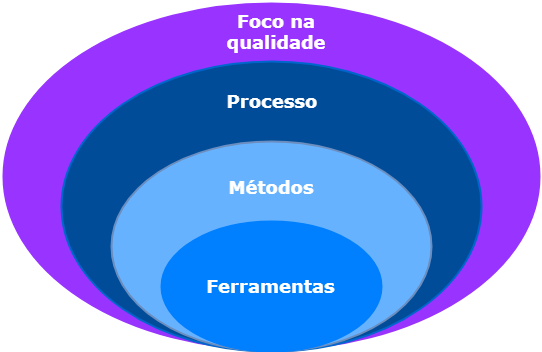
\includegraphics[scale=0.4]{figuras/camadas.png} % altere o atributo scale para o tamanho da figura
	\end{center}
	\label{fig:camadas}
	\legend{Fonte: Adaptado de \cite{pressman2005software}}
    \end{figure}
    
   Portanto, como a estrutura da sociedade hoje é dependente de sistemas computacionais, a engenharia de software é essencial nesse contexto. Esta área é responsável por cumprir estudos sobre como conhecer formas de construir, arquitetar e manter tais sistemas, tornando essencial no mundo moderno. Este trabalho é um estudo que está inserido na engenharia de software e se utilizará de conceitos da engenharia de requisitos. 
\end{comment}

     
\section{Engenharia de requisitos}

Visto que um software bem produzido é aquele que atende as necessidades do cliente, é necessário construir o sistema tendo um embasamento em fatos e informações reais. Sendo assim, a engenharia de requisitos é uma área da engenharia de software que pretende atingir esses objetivos. Esta área trata-se de um campo de estudo na engenharia de software de grande valia para o desenvolvimento de software.

    A engenharia de requisitos inclui atividades e etapas com o intuito de garantir que os requisitos reflitam as reais necessidades do solicitante. De acordo com \cite{kotonya}, o processo de engenharia de requisitos é composto por cinco etapas que são apresentadas na Figura \ref{fig:etapasRE}. 
    
    
    \begin{figure}[h!] %use h para forçar que a figura fique abaixo do texto
	\caption{Etapas da engenharia de requisitos.}
	\begin{center}
	    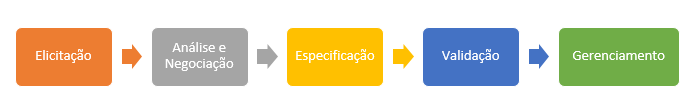
\includegraphics[scale=0.8]{figuras/ER} % altere o atributo scale para o tamanho da figura
	\end{center}
	\label{fig:etapasRE}
	\legend{Fonte: Adaptado de \cite{kotonya}.}
\end{figure}
    
    A elicitação consiste em identificar e coletar as informações e o escopo do projeto que serão refinados e classificados na etapa de análise e negociação. Na especificação, é realizado uma descrição das funcionalidades e restrições do sistema a partir do resultado da fase de análise. Na etapa de validação, os requisitos serão verificados se estão de acordo com as necessidades dos \emph{stakeholders}. Finalmente, a fase de gerenciamento aborda questões relacionadas a evolução e rastreamento dos requisitos.
    
    Por ser um processo dinâmico e eficiente, a engenharia de requisitos é adotada amplamente no desenvolvimento de software, suprindo desde o estudo de viabilidade até a elaboração do documento de requisitos. As práticas adotadas nesta fase do processo de desenvolvimento de software são indispensáveis e de benefícios imensuráveis para projetos e empresas.
    
    A definição de requisitos requer a comunicação e colaboração de diversos \emph{stakeholders}. O processo de comunicação é descrito na próxima seção.
\section{Teoria da comunicação} \label{sec:fund_comunicacao}

A teoria da comunicação é uma área de pesquisa bastante abrangente que diz respeito aos efeitos da comunicação em todo o meio tecnológico, social, entre outros. Esta teoria define dois aspectos distintos \cite{pernstal}: um referindo-se ao processo da comunicação em si sendo retratado na troca de mensagens entre duas partes; e o outro ao significado do conteúdo ou ideia que está sendo transmitida.

No primeiro caso, a comunicação é analisada como um processo de transferência de informações entre os indivíduos ou partes (por exemplo, pessoas, grupos, organizações, documentos, etc.). Apesar de existir vários processos para descrever a comunicação, existem os seguintes pontos em comum \cite{pernstal}:

\begin{itemize}
    \item Remetente - quem está enviando a mensagem? 
    \item Mensagem - o que está sendo comunicado?
    \item Receptor - quem é o destinatário da mensagem?
    \item Canal de comunicação - como a mensagem é transmitida?
    \item Efeito - o resultado final da comunicação.
\end{itemize}

Também é importante ressaltar os seguintes conceitos:

\begin{itemize}
    \item Codificação – é a forma como o pensamento é processado. É transformar a informação em algo conhecido que será transferido.
    \item Decodificação – processo pelo qual o receptor ``traduz'' a informação emitida pelo emissor. Essa tradução vai depender de diversos fatores sendo de crucial importância no processo.
\end{itemize}

Esses conceitos envolvidos na comunicação são ilustrados na Figura \ref{fig:processocomunicacao}. Um elementos adicional nesse processo de comunicação pode ser uma fonte de ruído que é o termo utilizado quando algo é capaz de mudar ou distorcer a mensagem original do remetente \cite{pernstal}. 

\begin{figure}[h!] 
   	    \captionsetup{width=13cm}%Da mesma largura que a figura
		\Caption{\label{fig:processocomunicacao} Exemplo processo de comunicação.}
		\UFCfig{}{
			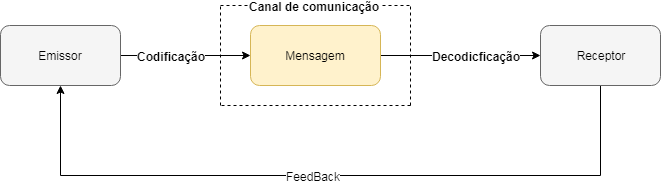
\includegraphics[width=13cm]{figuras/processoComunicacao.png}
		}{
			\Fonte{Fonte: Elaborado pelo autor }
		}	
	\end{figure}




A comunicação inserida no contexto de desenvolvimento de software é crucial para um projeto bem-sucedido \cite{pernstal, liskin2015artifacts}. A combinação da comunicação formal (por exemplo, documentos escritos e reuniões planejadas) e comunicação informal (por exemplo, reuniões presenciais não planejadas e outros meios convencionais como e-mails e redes sociais) interna e externamente em equipes, trata-se de um aspecto bastante vantajoso. 


\section{Comunicação de requisitos}

    A comunicação de requisitos se refere à capacidade das informações serem repassadas no processo de engenharia de requisitos, entre diferentes \emph{stakeholders}. Portanto, pode ser definida como a forma como o processo de comunicação atua na engenharia de requisitos. É de fundamental importância agilizar o processo. Quando a comunicação é falha, o projeto estará sujeito a atrasos, erros, ineficiência entre outros fatores.
    
Os canais de comunicação de requisitos são bastante variados podendo ser, por exemplo: 
    
\begin{itemize}
    \item Artefatos (documentos, modelos) gerados no processo;
    \item Ferramentas de comunicação;
    \item Reuniões (planejadas e não planejadas);
    \item Conversas informais e formais.
\end{itemize}

    Durante a comunicação, é crucial que a decodificação da informação seja correta para garantir a conformidade da mensagem recebida com a mensagem que espera-se ser passada. Portanto, a codificação têm de ser criteriosa e adequada para um bom entendimento.% sendo esses dois pontos que podem garantir a transferência das informações independente dos canais de comunicação. 
        
    O ambiente de comunicação de requisitos ideal seria onde todos os canais de comunicação permitissem passar as informações com o entendimento mútuo. Isto é, remetente e receptor em consenso sobre tal informação não havendo discordância, ambiguidade e incoerência sobre o efeito da informação repassada.


\section{Revisão sistemática da literatura} \label{sec:fund_slr}

Revisão sistemática da literatura, do inglês \emph{Systematic Literature Review} - SLR), trata-se de um tipo de pesquisa científica que reúne estudos relevantes ou trabalhos acadêmicos em relação a perguntas de pesquisa \cite{kitchenham}. Sendo assim, é um método empírico de pesquisa que define uma estratégia de busca de trabalhos que são selecionados por meio de critérios bem definidos.

Uma vez que um trabalho seja selecionado, são extraídas as informações requeridas para responder as perguntas de pesquisa. Em seguida, uma síntese dos dados é elaborada e, por fim, a publicação. Esses dados necessários para conduzir uma revisão sistemática são ilustrados na Figura \ref{fig:processoRevisao}.

\begin{figure}[h!]
	\caption{ Exemplo Processo de revisão sistemática.}
	\begin{center}
	    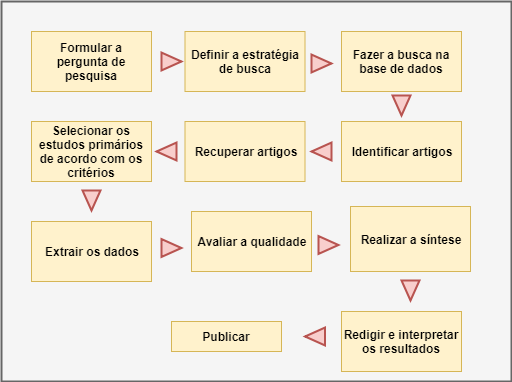
\includegraphics[scale=0.6]{figuras/sistematica.png}
	\end{center}
	\label{fig:processoRevisao}
	\legend{Fonte: Adaptado de \cite{kitchenham}.}
\end{figure}



A revisão sistemática da literatura é o método de pesquisa adotado neste trabalho para coleta dos dados. No próximo capítulo, a metodologia deste trabalho é descrita.

	\chapter{PROCEDIMENTOS METODOLÓGICOS}
\label{chap:metodologia}



%Procedimentos Metodológicos relaciona-se ao passo-a-passo da execução do trabalho pesquisa: como se obterá os dados necessários para respondem à sua questão de pesquisa? Um bom ponto de partida para escrever os procedimentos é detalhar extensamente cada objetivo específico.

%Para que os resultados encontrados sejam considerados válidos, é preciso respeitar e seguir as tradições de cada área de pesquisa. As estratégias de levantamento de dados, e de registro e análise do material coletado, mudam conforme a natureza da pesquisa. Seguem alguns exemplos:


A metodologia do trabalho adotou revisão sistemática da literatura \cite{kitchenham} como estratégia de pesquisa. Os trabalhos e dados relacionados aos fatores que influenciam a comunicação de requisitos na engenharia de software foram coletados. Para alcançar tal objetivo os passos ilustrados na Figura \ref{fig:metodologia} foram executados.

\begin{figure}[h!]
	\caption{Metodologia da pesquisa.}
	\begin{center}
	    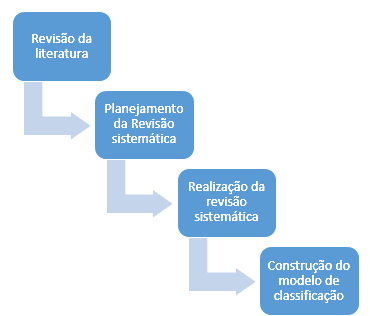
\includegraphics[scale=1.0]{figuras/metodologia}
	\end{center}
	\label{fig:metodologia}
	\legend{Fonte: Autor.}
\end{figure}
   
   
\section{Revisão da literatura}

    Como o objetivo deste trabalho foi identificar fatores de comunicação, em primeiro momento foi realizado uma revisão da literatura que consiste em uma pesquisa bibliográfica em trabalhos com conceitos em comum ou relacionados. Os estudos mais próximos com os objetivos desse trabalho foram descritos no Capítulo \ref{sec:objetivo-geral-2}. %resultando em um conjunto de trabalhos que serão posteriormente utilizados nos passos descritos nas seguintes seções. 
     
\section{Planejamento da Revisão Sistemática}

    Para a realização de revisões sistemática da literatura, foi necessário definir um protocolo de pesquisa. O protocolo da revisão seguido neste trabalho é descrito com detalhes na Seção \ref{sec:protocolo}.
    
    O protocolo foi desenvolvido seguindo as \emph{guidelines} de \cite{kitchenham}, explicadas na Seção \ref{sec:fund_slr}. A definição e execução da revisão sistemática foram suportadas pela ferramenta Parsifal \footnote{https://parsif.al/}. 
     
 \section{Realização da revisão Sistemática}  
 O protocolo definido foi seguido para obter estudos relacionados a comunicação de requisitos no processo de desenvolvimento de software. Esses estudos constituíram a fonte de dados para a obtenção dos fatores que influenciam a comunicação de requisitos.
 
    
%\subsection{Classificação dos fatores}

\section{Construção do modelo de classificação}

A partir dos fatores selecionados nos estudos provenientes da revisão sistemática, foi realizado então uma análise individual para identificar se a ocorrência do mesmo auxilia ou piora a comunicação. 

Com base no processo de comunicação (ver Figura \ref{fig:processocomunicacao}), foi identificado em qual ponto do processo cada fator obtido na revisão sistemática atua. Sabendo que no processo de comunicação envolvem os conceitos descritos na Seção \ref{sec:fund_comunicacao} (Codificação da informação, Decodificação da informação, Emissor, Receptor, Canal de comunicação, Mensagem e \emph{Feedback}), foi criado um modelo de classificação desses fatores. %Cada  para cada fa com "Seções" positivo, negativo.

%\begin{itemize}
%    \item Codificação da informação
%    \item Decodificação da informação
%    \item Emissor
%    \item Receptor 
%    \item Canal de comunicação 
%    \item Mensagem 
%    \item Feedback
%\end{itemize}



O modelo demonstra onde o fator atua no processo de comunicação e qual o impacto do mesmo, sendo este positivo ou negativo. Além disso, conceitos como os listados abaixo estão inclusos no modelo:

\begin{itemize} 
 \item Positivos: 
    \begin{itemize} 
        \item Melhoria 
        \item Boas práticas
    \end{itemize}

 \item Negativos: 
    \begin{itemize}
        \item Ruídos de comunicação
        \item Empecilhos e impedimentos 
    \end{itemize}
\end{itemize}

Como resultado foi proposto um modelo que demonstra onde os fatores atuam no processo de comunicação.


\begin{comment}
\section{Validação do modelo}
A validação do modelo ainda será planejada com detalhes, porém espera-se obter \emph{feedback} de profissionais e \emph{experts} em desenvolvimento de software da academia seguindo o modelo de transferência de tecnologia proposto por \cite{gorschekTechnology}. A validação será baseada em métodos e diretrizes de engenharia de software empírica \cite{wieringa} \cite{carolynqualitative}. Para conduzir a investigação com os profissionais, priorizar-se-á por aplicar uma abordagem de pesquisa qualitativa adotando entrevistas semiestruturadas como estratégia para alcançar os objetivos do estudo \cite{merriamqualitative}.
\end{comment}


%We followed the guidelines proposed by Runeson and Martin \cite{runeson} to investigate a contemporary phenomenon, i.e. the application of Uni-REPM SCS, within its real-life context (maturity evaluation of the companies). There are five major process steps to go through in the case study research process \cite{runeson} as presented in Figure \ref{fig:casestudysteps}.

\begin{comment}
\section{Cronograma de Execução}

Nesta seção será apresentado o cronograma de execução deste trabalho, ilustrado na seguinte tabela: 


\begin{table}[h!]
\centering
\resizebox{\textwidth}{!}{\begin{tabular}{|l|c|c|c|c|c|c|c|c|c|c|c|c|c|c|}
\hline
\multicolumn{1}{|c|}{\multirow{2}{*}{ATIVIDADES}} & \multicolumn{14}{c|}{2018} \\ \cline{2-15} 
\multicolumn{1}{|c|}{} & \multicolumn{2}{c|}{Mai} & \multicolumn{2}{c|}{Jun} & \multicolumn{2}{c|}{Jul} & \multicolumn{2}{c|}{Ago} & \multicolumn{2}{c|}{Set} & \multicolumn{2}{c|}{Out} & \multicolumn{2}{c|}{Nov} \\ \hline
\begin{tabular}[c]{@{}l@{}}
%Estudo de Domínio & x & x & x &  &  &  &  &  &  &  &  &  &  & - \\ \hline

Elaboração do protocolo da revisão sistemática\end{tabular} & x & x & x &  &  &  &  &  &  &  &  &  &  &  \\ \hline

Defesa do projeto &  &  &  & x &  &  &  &  &  &  &  &  &  &  \\ \hline

Condução da revisão sistemática &  &  &  &  & x & x & x & x &  &  &  &  &  &  \\ \hline

Construção do modelo &  &  &  &  &  &  &  & x &x  &x  &  &  &  &  \\ \hline

Validação do modelo &  &  &  &  &  &  &  &  &  &  & x & x &  &  \\ \hline

Análise dos resultados &  &  &  &  &  &  &  &  &  &  &x  &x  &x  &  \\ \hline

Escrita da monografia &  &  &  &  &  &  &  &  &  &  &  & x & x &  \\ \hline

Defesa do Trabalho Final &  &  &  &  &  &  &  &  &  &  &  &  &  & x \\ \hline
\end{tabular}}
\end{table}

No próximo capítulo é descrito o protocolo da revisão sistemática que será utilizado neste trabalho.
\end{comment}


	
\chapter{PROTOCOLO DA REVISÃO SISTEMÁTICA}
\label{sec:protocolo}       

O protocolo de uma revisão sistemática da literatura especifica os métodos que serão empregados para realizar a revisão. De acordo com \cite{kitchenham}, um protocolo bem definido é necessário para reduzir a possibilidade de viés do pesquisador. Por exemplo, sem um protocolo, é possível que a seleção de
estudos ou a análise seja conduzida segundo as expectativas do pesquisador. Nas próximas seções, são descritos os campos desse protocolo.

A definição do protocolo utilizado nessa pesquisa seguiu as \textit{guidelines} de \cite{kitchenham}. O protocolo, que foi definido utilizando a ferramenta \textit{Parsifal}, é detalhado nas próximas seções.

\section{Definição do objetivo} 
    
O objetivo desta revisão é identificar estudos que descrevam fatores que influenciam a comunicação de requisitos no processo de desenvolvimento de software.
%diretamente ou indiretamente na comunicação de requisitos.


\section{Perguntas de Pesquisa} \label{sec:RQs}


O critério PICOC (População, Intervenção, Comparação, Resultado e Contexto), do inglês \emph{Population, Intervention, Comparison, Outcome, Context}, foi utilizado para direcionar a definição das perguntas de pesquisa. 

\begin{itemize}
\item\textbf{População:} Publicações revisadas aos pares que descrevem fatores que influenciam a comunicação de requisitos no processo de desenvolvimento de software.
\item\textbf {Intervenção:} Coletar evidências empíricas em relação aos fatores que influenciam a comunicação de requisitos.
\item\textbf {Comparação:} Não se aplica, pois os estudos primários não serão comparados. 
\item\textbf {Resultados:} Respostas para as perguntas de pesquisa.
\item\textbf {Contexto:} Engenharia de Software desde que \emph{stakeholders} comuniquem requisitos.
\end{itemize}

Considerando o objetivo dessa revisão e o critério PICOC, pretende-se responder as perguntas de pesquisa apresentadas na Tabela \ref{tab:rqs}.

        \begin{table}[h!]
        \centering
        \caption{Perguntas de pesquisa.}
        \begin{tabular}{p{12cm}}
        
        \hline
        
P1. Quais são os stakeholders envolvidos? \\\hline
P2. Quais são os problemas de comunicação reportados no estudo?\\\hline
P3. Quais são os fatores de comunicação apontados no estudo?\\\hline
P4. Qual o impacto do fator de comunicação?\\\hline
P5. O fator interfere em qual aspecto do processo de comunicação?\\\hline


        \label{tab:rqs}
        \end{tabular}
         \legend{Fonte: Elaborado pelo autor}
        \end{table}        

\section{String de Busca}

A \emph{string} de busca foi definida considerando os principais termos dos conceitos sob investigação. As palavras-chave são listadas na Tabela \ref{tab:keywords}.

        \begin{table}[h!]
        \centering
        \caption{Palavras chave.}
        \label{tab:keywords}
        \begin{tabular}{p{5cm}p{9cm}}
        \hline
        \textbf{Conceito}  & \textbf{Palavras-chave}   \\ \hline
        Problemas de comunicação                               & Communication Challenges, Communication Risk, Requirements Issues, Requirements communication       \\ \hline
        Fatores & Factor, Action, Characteristic, Feature, Practice \\ \hline
        Requirement &Requirement, Functional Requirement, Functionality \\\hline
        
        \end{tabular}
         \legend{Fonte: Elaborado pelo autor}
        \end{table}
  
        Pesquisas piloto foram realizadas de maneira iterativa para refinar a \emph{string} de busca. Foram excluídas palavras-chave cuja inclusão não retornou documentos adicionais nas pesquisas automáticas. Após várias iterações, a seguinte \emph{string} foi usada para pesquisar nas palavras-chave, título, resumo e texto completo das publicações:

\emph{        
(“communication challenge” OR “communication problem” OR “communication
risk” OR “requirements issue” OR “requirements communication”) AND (“factor” OR “action”
OR “characteristic” OR “feature” OR "practice”) AND (“software engineering”) AND (“software
development”) AND (“requirement” OR “functional requirement” OR “functionality”)
}
\newpage

\section{Bases de dados}\label{sec:bases}

As bases de dados que foram utilizadas para a seleção dos artigos são descritas na Tabela \ref{tab:bases}.


\begin{table}[h]
\centering
\caption{Bases utilizadas na pesquisa.}
\begin{center}
\scriptsize
\label{base_de_pesquisa}
\begin{tabular}{p{5.0cm}p{5.0cm}}
\hline

\textbf{Nome}
&\textbf{URL}\\

\hline
ACM Digital Library &	http://portal.acm.org\\ 
IEEE Digital Library &	http://ieeexplore.ieee.org\\ 
Science@Direct &	http://www.sciencedirect.com \\	 
Scopus &	http://www.scopus.com \\
\hline
 
\end{tabular} 

\legend {\fontsize{10}{12}\selectfont {Fonte: Autor.}}
\end{center}
\label{tab:bases}
\end{table}


       \section{Critérios de seleção}
        \label{sec:criterios}
        
            Os critérios de seleção foram utilizados para determinar se um trabalho deve ou não ser incluído na revisão. Esses critérios estão descritos na Tabela \ref{tab:criterios}.
        
\begin{comment}

\begin{itemize}
            \item Estudos primários.
               \item Estudos publicado em qualquer ano até julho de 2018.
               \item Estudos que abordam nos objetivos comunicação de requisitos. 
               \item Estudos que relacionam requisitos e comunicação.
              
           \end{itemize}
    
            Da mesma forma, será adotado os seguintes critérios para exclusão:
      
            \begin{itemize}
                \item Artigos curtos (\emph{short papers}) com menos de quatro páginas.
                \item Estudos duplicados.
                \item Estudos incompletos.
                \item Estudos secundários.
                \item Estudos redundantes da mesma autoria.
                \item Estudos claramente irrelevantes para a pesquisa, levando em consideração as questões de pesquisa.
                \item Estudos cujo foco não se relaciona a comunicação de requisitos.
                \item Estudos cujo texto não esteja disponível.
                \item Literatura cinza (teses, dissertações, monografias, etc).
                \item Estudos não escritos em inglês.
            \end{itemize}
            
\end{comment}            
        

        \begin{table}[h!]
        \centering
        \caption{Critérios de inclusão e exclusão.}
        \label{tab:criterios}
        \footnotesize
        \begin{tabular}{p{6cm}p{6cm}}
        \hline
        \textbf{Critérios de inclusão}  & \textbf{Critérios de exclusão}   \\ \hline
        Estudos primários                               & Estudos curtos (\emph{short papers}) com menos de quatro páginas.       \\ \hline
        Estudos publicados em qualquer ano até julho de 2018. & Estudos duplicados. \\ \hline
        Estudos que abordam nos objetivos comunicação de requisitos.  &Estudos incompletos. \\\hline
        Estudos que relacionam requisitos e comunicação.  & Estudos secundários. \\\hline
        
        Estudos que respondam alguma pergunta de pesquisa.   & Documento redundante da mesma autoria.\\\hline
                                                         & Estudos claramente irrelevantes para a pesquisa, levando em consideração as questões de pesquisa.\\\hline
                                                         & Estudos cujo foco não relaciona-se a comunicação de requisitos.\\\hline
                                                         & Estudos cujo texto completo não esteja disponível.\\\hline
                                                         & Literatura cinza (teses, dissertações, monografias, etc).\\\hline
                                                         & Estudos não escritos em inglês.\\\hline
                                                        
        
        \end{tabular}
        \legend{Fonte: Elaborado pelo autor}
        \end{table}
  \begin{comment}
  
  \section{Critérios de avaliação de qualidade}
        
        A avaliação da qualidade é crítica em uma revisão sistemática para investigar se diferenças de qualidade nos artigos selecionados fornecem uma explicação para as diferenças nos resultados obtidos \cite{kitchenham}. Este trabalho considera que a qualidade se relaciona com a medida em que o estudo minimiza o viés e maximiza a validade e credibilidade, por meio dos critérios descritos na Tabela \ref{tab:quality}.
        
       
\begin{table*}[h!]
 \centering
     \scriptsize
 \caption{Critérios de avaliação da qualidade do estudo.}
 \begin{tabular}{p{10cm}p{0.5cm}p{0.5cm}p{0.5cm}p{0.5cm}p{0.5cm}}
 \hline
 \textbf{Critério} & \textbf{Eva}	& \textbf{Val} & \textbf{Sol} & \textbf{Exp} & \textbf{Op}\\
 \hline
 Q1. Possui uma declaração clara dos objetivos da pesquisa? &x	&x	&x	&x\\
 \hline
Q2. A técnica proposta é  descrita claramente? & & &x	& \\
 \hline
 Q3. Há uma descrição adequada do contexto (indústria, ambiente de laboratório, produtos utilizados e assim por diante) em que a pesquisa foi realizada? 	&x	&x	& & \\
 \hline	





Q1. Existe discussão sobre os resultados do estudo? 	&x	&x	&x &\\
 \hline	
Q2. As limitações do artigo são explicitamente discutidas? &x	&x	&x	&\\
 \hline
Q3. As lições aprendidas são interessantes? & & & &x\\
 \hline
Q4.  O artigo é relevante para os profissionais da indústria?	&x	&x	&x	&x\\
 \hline
Q5. Há discussão suficiente sobre trabalhos relacionados? (As técnicas concorrentes são discutidas e comparadas com a técnica atual?)	&x	&x	&x	&\\
 \hline
Q6. Os participantes do estudo ou unidades de observação são descritos adequadamente? Por exemplo, experiência em Engenharia de Software, tipo (estudante, profissional, consultor), nacionalidade, experiência em tarefas e outras variáveis relevantes. &x	&x & &\\
 \hline		

Q7. O estudo amplia suficientemente o conhecimento sobre comunicação de requisitos no processo de desenvolvimento de software?	&x	&x	&x	&x\\
 \hline	
Q8. O posicionamento sobre o tema é adequado?	&	&	&	& & x\\
 \hline	
Q9. É provável que provoque discussão sobre o tema?	&	& &  &	&x\\
 \hline	

Q10. Quão claras são as hipóteses/concepções teóricas/valores que moldaram as configurações e as opiniões descritas?	&	&	&	& & x\\
 \hline
 \end{tabular}%
 \legend{Fonte: Adaptado de \cite{vilela2017integration}.}
 \label{tab:quality}%
\end{table*}%

        A avaliação da qualidade dos artigos foi realizada por meio de uma técnica de pontuação para avaliar a credibilidade, completude e relevância dos estudos selecionados. Os artigos serão avaliados em relação a um conjunto de 10 critérios de qualidade proposto por \cite{vilela2017integration}.
        
        O trabalho diferencia os estudos em cinco categorias: artigos de avaliação (\emph{Evaluation Research Papers} - EVA); artigos de validação (\emph{Validation Research} Papers - VAL); Propostas de solução (\emph{Solution Proposal Papers} - SOL); Relatos de experiência (\emph{Experience Papers} - EXP); e artigos de opinião (\emph{Opinion Papers} - OP). %Os critérios são descritos na Tabela \ref{tab:quality}.
        
        Cada critério da avaliação de qualidade possui três respostas possíveis: ``Sim'' (pontuação = 1), ``Parcialmente'' (pontuação = 0,5) ou ``Não'' (pontuação = 0). Consequentemente, o grau de qualidade de um artigo é calculado considerando a soma das pontuações das respostas para as questões relacionadas ao seu tipo de pesquisa.
\end{comment}  
   
\section{Formulário de extração de dados}
    
     Para guardar todas as informações necessárias para responder às perguntas da pesquisa foi preparado o formulário de extração de dados apresentado na Tabela \ref{tab:extraction}.
    
    \begin{table}[h]
    \centering
    \scriptsize
    \caption{Formulário de extração dos dados.}
    \label{tab:extraction}
    \begin{tabular}{p{5cm}p{6cm}p{4cm}}
    \hline
    \textbf{Dado} & \textbf{Descrição}  & \textbf{Pergunta de Pesquisa}\\ \hline
    Autores, ano, título     &  &Visão Geral dos estudos  \\ \hline
    Origem do trabalho       & IEEE, ACM, Springer, Scopus, Science Direct    \\ \hline
  
   Stakeholders envolvidos & &P1  \\ \hline
    
    Fator  de comunicação   & &P2 \\ \hline
    
    Impacto do fator de comunicação & &P3 \\ \hline
   
    Aspecto do processo de comunicação afetado & &P4 \\ \hline
   
    Canal de comunicação utilizado & &P5 \\ \hline
   
  
    \end{tabular}
    \legend{Fonte: Elaborado pelo autor.}
    \end{table}
        
\section{Procedimento para seleção de estudos}

        O procedimento de seleção de estudos consistiu em cinco etapas principais. Na primeira, os estudos foram consultados e obtidos por meio de busca automática usando a \emph{string} de pesquisa nas bases de dados apresentadas na Tabela \ref{tab:bases}. Os resultados das buscas foram armazenados na ferramenta Parsifal.

        A segunda etapa consistiu na eliminação de artigos duplicados. Em seguida, no passo 3, houve a seleção dos estudos primários obtidos na etapa anterior por meio da leitura de título e \emph{abstract} usando os critérios de inclusão e exclusão descritos na Seção \ref{sec:criterios}. Se houve dados insuficientes ou dúvidas, o artigo seguiu para o próximo passo.
        
        O quarto passo consistiu na leitura completa dos artigos para responder as perguntas de pesquisa usando o formulário de extração da Tabela \ref{tab:extraction}.
      
    \section{Ameaças à validade} 
        
        A classificação de ameaças à validade descrita por \cite{Wohlin2000} foi utilizada para discutir as ameaças deste trabalho. Esta classificação define quatro tipos de ameaças de validade, sendo elas, ameaças de conclusão, internas, de construção e de validade externa.
        
        \emph{Ameaças à validade de constructo:} Este tipo de validade diz respeito à generalização do resultado para o conceito ou teoria por trás da execução do estudo. Com o objetivo de minimizar ameaças dessa natureza, foi utilizado sinônimos para as principais palavras chaves.
        
       \emph{Ameaças de validade interna:} estão relacionadas a uma possível conclusão errada sobre as relações causais entre o tratamento e o resultado \cite{Wohlin2000}. Decisões subjetivas podem ocorrer durante a seleção de artigos e extração de dados uma vez que é comum estudos primários não fornecerem uma descrição clara ou objetivos e resultados apropriados, dificultando a aplicação objetiva dos critérios de inclusão/exclusão ou a imparcialidade. A fim de minimizar erros de seleção e extração, o processo de seleção foi realizado de forma iterativa de forma que quando ocorreu dúvida na aplicação de algum critério, o estudo não foi eliminado e passou para a próxima fase. Além disso, o processo de seleção foi realizado de forma colaborativa pelo autor e por um colaborador de forma que conflitos foram discutidos e solucionados pelos mesmos em conjunto com a orientadora. Dessa forma, objetivou-se atenuar as ameaças devido ao viés pessoal na compreensão do estudo.
        
        \emph{Ameaças à validade externa:} está relacionada ao grau em que os estudos primários serão representativos para o tópico de revisão. Se tratando de uma revisão da literatura, a validade externa depende da literatura identificada: se a literatura identificada não é valida externamente, tampouco a síntese do seu conteúdo é citada. Esta ameaça foi mitigada devido a utilização do critério de exclusão para eliminar, da pesquisa, os estudos provenientes de literatura cinza. Além disso, para mitigar as ameaças externas, o protocolo de pesquisa foi definido iterativamente e, validado, com o consenso do autor, do colaborador e da orientadora.  
        
        \emph{Ameaças à validade de conclusão}: A metodologia descrita por \cite{kitchenham} assume que nem todos os estudos primários relevantes possam vir a ser identificados. Para amenizar os efeitos dessa ameaça, o processo da revisão foi cuidadosamente elaborado e discutido pelos autores para minimizar o risco de exclusão estudos relevantes. Outro método empregado foi utilizar expressões e palavras sinônimas para os constructos dessa revisão sistemática, essa técnica objetiva uma maior cobertura de estudos possivelmente importantes a partir da pesquisa automática. Além disso, o processo de seleção do estudo foi conduzido em paralelo e de forma independente pelo aluno e pelo colaborador. Posteriormente, os resultados foram harmonizados para mitigar o viés pessoal na seleção do estudo causado por revisores individuais. Finalmente, a orientadora supervisionou esse processo.
        
        Para minimizar ameaças no processo de seleção dos estudos calculou-se um índice de concordância na etapa de classificação de artigos, feito junto a um colaborador e o autor do estudo, Os resultados obtidos foram satisfatórios visto que o menor número de concordância obtido foi 85\% e estão ilustrados na Tabela \ref{tab:concord}.
        
        
        \begin{table}[h!]
        \caption{Índice de concordância}
        \label{tab:concord}
\begin{tabular}{|l|l|l|l|l|l|}
\hline
\textbf{Base} & \textbf{Artigos} & \textbf{Duplicados} & \textbf{Autor Rejeitou} & \textbf{Colaborador Rejeitou} & \textbf{Concordância} \\ \hline
ACM           & 8                & 3                   & 4                      & 4                           & 100\%                 \\ \hline
IEEE          & 211              & 17                  & 161                    & 163                         & 92,2\%                \\ \hline
SCIENCE       & 324              & 16                  & 274                    & 255                         & 85,7                  \\ \hline
SCOPUS        & 317              & 41                  & 241                    & 220                         & 90,4                  \\ \hline
\end{tabular}
 \legend{Fonte: Elaborado pelo autor}
\end{table}
        
        
        
        
O próximo capítulo apresenta a condução da revisão sistemática.      

\newpage

\begin{comment}ou mapeamento sistematico
%bolsista
\begin{alineascomponto}
    \item Escolha de trabalhos;
    \item Definição dos critérios;
    \item Identificação se existe algum fator;
    \item Classificação dos fatores;
    \item Construção do modelo de classificação;
    \item Validação do modelo;

\end{alineascomponto}

%, lembrando que alguns passos serão executados em duas partes, duas pessoas diferentes para obtenção de dados mais confiáveis e maior credibilidade.

\section{Escolha de trabalhos}

Para que um trabalho seja escolhido e relacionado será feita uma primeira triagem selecionando entre trabalhos relacionados á desenvolvimento de software e coletando os que possuem palavras-chave que estejam diretamente relacionadas com o tema, abrangendo também outras palavras chaves que poderão ser úteis para a coleta dos fatores mesmo que no devido trabalho não haja um relacionamento explícito.

Palavras chaves diretas:
\begin{itemize}
    \item Comunicação
    \item Problemas de comunicação 
    \item Otimização de comunicação
    \item Comunicação de requisitos
    \item Engenharia de requisitos 
    \item Artefatos de requisitos
    \item Boas práticas
\end{itemize}

Nos trabalhos com as seguintes palavras chaves será buscado se há relacionamento mesmo que indireto com comunicação

Palavras chaves de relacionamento indireto:
\begin{itemize}
    \item Melhoria de processo 
    \item Metodologias de otimização
    \item Levantamento de boas práticas
\end{itemize}


\subsection{Definição dos critérios}

Os critérios de seleção são descritos como algo que afeta diretamente ou indiretamente a comunicação de requisitos independente do que se trata.

Critérios:

\begin{itemize}
    \item Afeta positivamente a comunicação ?
    \item Afeta negativamente a comunicação ?
    \item Otimiza o processo de comunicação ?
    \item Ocasiona ruído de comunicação ? 
    \item Descreve prática relacionado a comunicação ?
    \item Descreve metodologia relacionado a comunicação ?
\end{itemize}

\section{Identificação se existe algum fator}

Com os critérios de seleção definidos iremos verificar se o trabalho selecionado  descreve algum problema, melhoria, otimização ou identifica algo que está relacionado direto ou indiretamente a comunicação inserido no contexto do desenvolvimento de software, se sim iremos decidir se  tal informação é um fator que pode influenciar no processo de comunicação, ressaltando que para a informação seja selecionada é necessário que atenda a um ou mais dos critérios descritos na etapa anterior.

\section{Classificação dos fatores}

Com os fatores selecionados será feito então uma análise individual entre os fatores para identificar se a ocorrência do mesmo auxilia, impede, melhora ou piora a comunicação. 

\section{Avaliação de qualidade} 

A avaliação da qualidade é crítica em uma revisão sistemática para investigar se diferenças de qualidade nos artigos selecionados fornecem uma explicação para as diferenças nos resultados obtidos \cite{kitchenham}. Seguindo as diretrizes desses autores, este trabalho considera que a qualidade se relaciona com a medida em que o estudo minimiza o viés e maximiza a validade interna e externa.

A avaliação da qualidade dos artigos selecionados será realizada por meio de uma técnica de pontuação para avaliar a credibilidade, completude e relevância dos estudos selecionados. Os artigos serão avaliados em relação a um conjunto de 20 critérios de qualidade proposto por \cite{vilela2017integration}.

O trabalho de diferencia os estudos em cinco categorias: artigos de avaliação (Evaluation Research Papers - EVA); artigos de validação (Validation Research Papers - VAL); Propostas de solução (Solution Proposal Papers - SOL); Relatos de experiência (Experience Papers - EXP); e artigos de opinião (Opinion Papers - OP). Os critérios são descritos na Tabela \ref{tab:quality}.

Cada critério da avaliação de qualidade possui três
respostas possíveis: ``Sim" (pontuação = 1), ``Parcialmente'' (pontuação = 0,5) ou ``Não'' (pontuação = 0). Consequentemente, o grau de qualidade de um artigo é calculado considerando a soma das pontuações das respostas para as questões relacionadas ao seu tipo de pesquisa. A maior pontuação que um artigo poderá obter será 100\% ou seja 20 pontos, e a pontuação mínima para o artigo ser analisado nessa revisão sistemática será de 50\%, ou seja 10 pontos.

\begin{table*}[h!]
 \centering
     \scriptsize
 \caption{Critérios de avaliação da qualidade do estudo.}
 \begin{tabular}{p{10cm}p{0.5cm}p{0.5cm}p{0.5cm}p{0.5cm}p{0.5cm}}
 \hline
 \textbf{Critério} & \textbf{Eva}	& \textbf{Val} & \textbf{Sol} & \textbf{Exp} & \textbf{Op}\\
 \hline
 Q1. Possui uma declaração clara dos objetivos da pesquisa? &x	&x	&x	&x\\
 \hline
Q2. A técnica proposta é  descrita claramente? & & &x	& \\
 \hline
 Q3. Há uma descrição adequada do contexto (indústria, ambiente de laboratório, produtos utilizados e assim por diante) em que a pesquisa foi realizada? 	&x	&x	& & \\
 \hline	
Q4. Os tratamentos foram alocados aleatoriamente? &	x & & & 	\\
 \hline		
Q5. A amostra é representativa do público para a qual os resultados serão generalizados? &x	&x	& & \\
 \hline	
Q6. Havia algum grupo de controle presente com o qual os tratamentos pudessem ser comparados, se aplicáveis?	&x	& & &	\\
 \hline	
Q7. Caso tenha um grupo de controle, os participantes são semelhantes aos do grupo de tratamento em termos de variáveis que podem afetar os resultados obtidos? 	&x	& & &			\\
 \hline
Q8. A análise de dados foi rigorosa o suficiente?	&x	&x	& & \\
 \hline	
Q9. Existe discussão sobre os resultados do estudo? 	&x	&x	&x &\\
 \hline	
Q10. As limitações do artigo são explicitamente discutidas? &x	&x	&x	&\\
 \hline
Q11. As lições aprendidas são interessantes? & & & &x\\
 \hline
Q12.  O artigo é relevante para os profissionais da indústria?	&x	&x	&x	&x\\
 \hline
Q13. Há discussão suficiente sobre trabalhos relacionados? (As técnicas concorrentes são discutidas e comparadas com a técnica atual?)	&x	&x	&x	&\\
 \hline
Q14. Os participantes do estudo ou unidades de observação são descritos adequadamente? Por exemplo, experiência em Engenharia de Software, tipo (estudante, profissional, consultor), nacionalidade, experiência em tarefas e outras variáveis relevantes. &x	&x & &\\
 \hline		
Q15. Existe evidências de cuidados com as considerações éticas?	&x	&x	& &	\\
 \hline
Q16. O estudo amplia suficientemente o conhecimento sobre ferramentas colaborativas no desenvolvimento do software?	&x	&x	&x	&x\\
 \hline	
Q17. O posicionamento sobre o tema é adequado?	&	&	&	& & x\\
 \hline	
Q18. É provável que provoque discussão sobre o tema?	&	& &  &	&x\\
 \hline	
Q19. Quão bem a diversidade de perspectiva e o contexto foram explorados? 	&	&	&	& & x\\
 \hline	
Q20. Quão claras são as hipóteses/concepções teóricas/valores que moldaram as configurações e as opiniões descritas?	&	&	&	& & x\\
 \hline
 \end{tabular}%
 \label{tab:quality}%
\end{table*}%

\section{Procedimento para seleção de estudos}

O procedimento de seleção de estudos, apresentado na Figura consistirá em cinco etapas principais. Na primeira, os estudos serão consultados e obtidos por meio de busca automática usando a \emph{string} de pesquisa nas bases de dados apresentadas na Tabela \ref{tab:bases}. Os resultados das buscas serão armazenados na ferramenta Parsifal.

A segunda etapa consistirá na eliminação de artigos duplicados. Em seguida, no passo 3, haverá a seleção dos estudos primários obtidos na etapa anterior por meio da leitura de título e \emph{abstract} usando os critérios de inclusão e exclusão descritos na Seção \ref{sec:criterios}. Se houver dados insuficientes ou dúvidas, o artigo seguirá para o próximo passo.

O quarto passo consistirá na leitura completa dos artigos para responder as perguntas de pesquisa descritas na Seção \ref{sec:perguntas} usando o formulário de extração da Tabela \ref{}.

Finalmente, será realizada a avaliação da qualidade dos artigos usando os critérios da Tabela \ref{tab:quality}.

\section{Ameaças à validade}

We used the categorization of threats presented by Wholin et. al \cite{Wohlin2000}, which includes four types of validity threats, namely, conclusion, internal, construct, and external validity threats. 

\emph{Construct validity}: Construct validity is related to generalization of the result to the
concept or theory behind the study execution \cite{Wohlin2000}. Aiming to minimize threats of this nature, we used many synonyms for the main constructs in this review: ``safety-critical systems'', ``requirements engineering'', ``safety requirements'', and ``communication''. 

\emph{Internal validity} threats are related to possible wrong conclusion about causal relationships between treatment and outcome \cite{Wohlin2000}. The primary objective of conducting a SLR is to minimize internal validity threats in the research. Decisões subjetivas podem ocorrer durante a seleção de artigos e extração de dados uma vez que é comum estudos primários não fornecerem uma descrição clara ou objetivos e resultados apropriados, dificultando a aplicação objetiva dos critérios de inclusão/exclusão ou a imparcialidade. A fim de minimizar erros de seleção e extração, o processo de seleção será realizado de forma iterativa de forma que quando ocorrer dúvida na aplicação de algum critério, o estudo não será eliminado e passará para a próxima fase. Além disso, o processo de seleção será realizado de forma colaborativa pela aluno e por um colaborador de forma que conflitos sejam discutidos e solucionados pelos alunos em conjunto com a orientadora. Dessa forma, objetiva-se atenuar as ameaças devido ao viés pessoal na compreensão do estudo.

\emph{External validity} is concerned with establishing the generalizability of the SLR results, which is related to the degree to which the primary studies are representative for the review topic. In the case of a literature review, the external validity depends on the identified literature: if the identified literature is not externally valid, neither is the synthesis of its content \cite{gasparic2016recommendation}. Esta ameaça será mitigada devido a utilização do critério de exclusão para eliminar, da pesquisa, os estudos provenientes de literatura cinza. Além disso, para mitigar as ameaças externas, o protocolo de pesquisa foi definido iterativamente e, validado, com o consenso da autora, do colaborador e da orientadora. Esta ameaça será mitigada devido a utilização do critério de exclusão para eliminar, da pesquisa, os estudos provenientes de literatura cinza. Além disso, para mitigar as ameaças externas, o protocolo de pesquisa foi definido iterativamente e, validado, com o consenso da autora, do colaborador e da orientadora.

\emph{Conclusion validity}: The used methodology of Kitchenham and Charters \cite{kitchenham} already assumes that not all relevant primary studies that exist can be identified. nem todos os estudos primários que existem  relacionados à pesquisa podem ser identificados, sendo assim, para minimizar esse ameaça, o processo da revisão foi cuidadosamente elaborado e discutido pelos autores para minimizar o risco de exclusão
estudos relevantes. Outro método empregado foi utilizar expressões e palavras sinônimas para os constructos dessa revisão sistemática, essa técnica objetiva uma maior cobertura de estudos possivelmente importantes a partir da pesquisa automática. Além disso, o processo de seleção do estudo será conduzido em paralelo e de forma independente entre autor e pelo colaborador. Posteriormente, os resultados serão harmonizados para mitigar o viés pessoal na seleção do estudo causado por revisores individuais. Finalmente, a orientadora supervisionará esse processo.

\end{comment}
	\chapter{Resultados}

O processo de seleção dos estudos, apresentado na Figura \ref{fig:dist}, consistiu em quatro etapas principais. Dos 860 resultados de pesquisa, 783 eram únicos (passo 2, Figura \ref{fig:dist}). Posteriormente, lendo o título e o resumo dos artigos, foram excluídos 673 estudos, baseados nos critérios de exclusão (passo 3). Quando não havia dados suficientes para exclusão, o trabalho foi deixado para o próximo passo. Depois de terminar o passo 3, 110 trabalhos permaneceram no processo de seleção. Depois de ler e analisar os 110 artigos deixados para a leitura de texto completo (passo 4), obtivemos 94 artigos relevantes. 

\begin{figure}[h!] %use h para forçar que a figura fique abaixo do texto
	\caption{Distribuição dos trabalhos na revisão.}
	\begin{center}
	    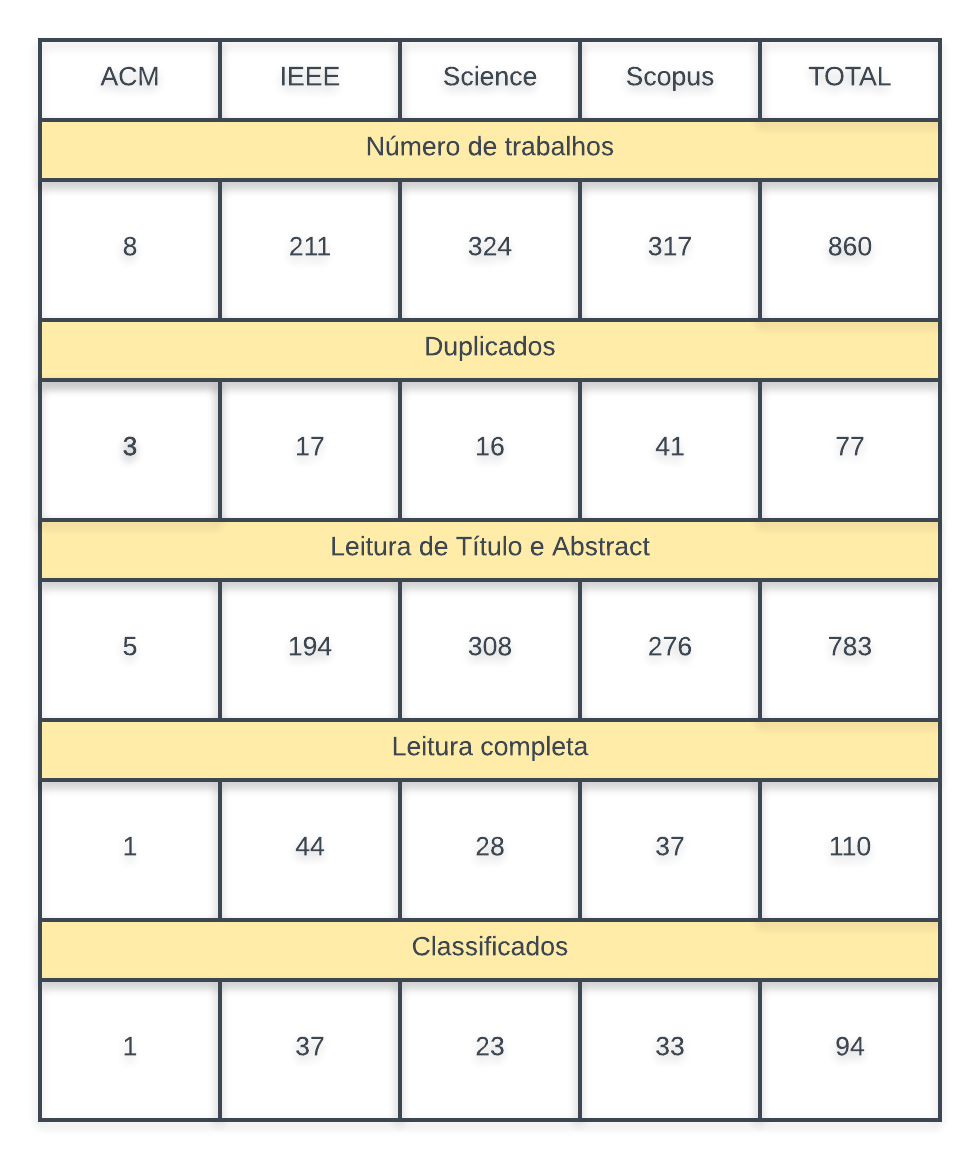
\includegraphics[scale=0.3]{figuras/revvisao.png} % altere o atributo scale para o tamanho da figura
	\end{center}
	\label{fig:dist}
	\legend{Fonte: Elaborado pelo autor.}
\end{figure}

\begin{comment}

\section{Avaliação de Qualidade}
   descritos na tabela \ref{tab:quality} cada critério podendo responder a três opções "Sim", "Não", "Parcialmente" sobre o dado relevante para a pesquisa, opções essas que impactam na pontuação geral do trabalho em respectiva ordem 1.0, 0.0, 0.5 cada trabalho podendo atingir um máximo de 12 e o mínimo em 5.0. Felizmente, nenhum trabalho foi excluído do estudo pela pontuação na avaliação de qualidade.
\end{comment} 


Os dados foram extraídos dos 94 estudos que satisfizeram os critérios de inclusão seguindo o formulário de extração descrito na Tabela \ref{tab:extraction}. Antes de apresentar os resultados e análises das perguntas de pesquisa, é fornecido uma visão geral das características gerais dos estudos.
\section{Visão geral dos estudos}

As bases de dados retornaram um total de 860 trabalhos sendo distribuídos em ACM: 8, IEEE: 211, Science: 324, Scopus: 317, a
disposição dos mesmos está ilustrada na Figura \ref{fig:grafartigosbase}.


\begin{figure}[h!] 
   	    \captionsetup{width=16cm}%Da mesma largura que a figura
		\Caption{\label{fig:grafartigosbase} Artigos por base.}
		\UFCfig{}{
			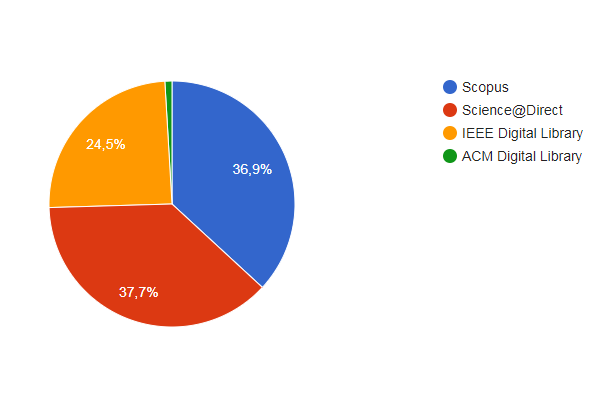
\includegraphics[width=13cm]{figuras/artigosbase}
		}{
			\Fonte{Ferramenta Parsif.al.}
		}	
	\end{figure}
Os trabalhos aceitos por cada base totalizaram 94 sendo distribuídos: ACM: 1, IEEE: 37, Science: 23, Scopus: 33, ver Figura \ref{fig:grafartigosacc}.


\begin{figure}[h!] 
   	    \captionsetup{width=16cm}%Da mesma largura que a figura
		\Caption{\label{fig:grafartigosacc} Artigos aceitos por base.}
		\UFCfig{}{
			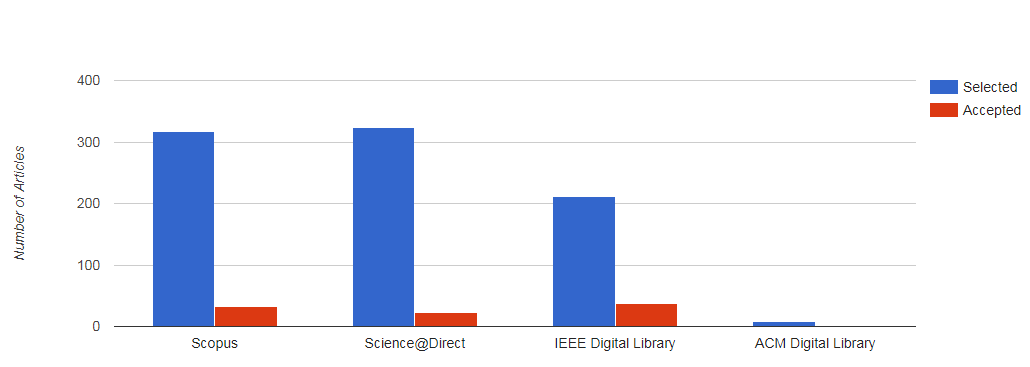
\includegraphics[width=13cm]{figuras/artigosbase1}
		}{
			\Fonte{Ferramenta Parsif.al.}
		}	
	\end{figure}



Constatou-se a importância da comunicação no âmbito da indústria e na academia, e o quão é notável que a pesquisa na comunicação no desenvolvimento de software é algo recorrente que cresceu ao longo dos anos como indica a figura que representa os anos de publicação dos trabalhos avaliados no estudo (ver Figura \ref{fig:camadas}).



\begin{figure}[h!] 
   	    \captionsetup{width=16cm}%Da mesma largura que a figura
		\Caption{\label{fig:camadas} Ano de publicação dos trabalhos.}
		\UFCfig{}{
			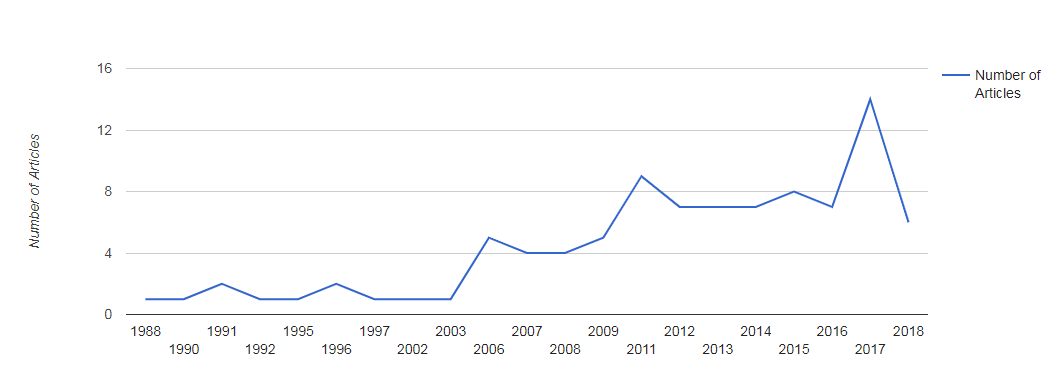
\includegraphics[width=16cm]{figuras/artigosbase2}
		}{
			\Fonte{Ferramenta Parsif.al.}
		}	
	\end{figure}


A extração dos dados mostrou que a pesquisa na área de comunicação de requisitos é relevante, a tabela a seguir contém autores de pelo menos três artigos avaliados neste estudo.

\begin{table}[h!]
\label{tab:autores1}
\caption{Autores com três ou mais trabalhos avaliados neste estudo.}
\begin{tabular}{|p{5cm}|p{9cm}|}
\hline
\textbf{Autores}                                     &                  \textbf{Referências}                                                                                                               \\ \hline
Kai Stapel                                          &

\cite{Stapel} 
\cite{stapel2011flow}
\cite{knauss2013v}
\cite{knauss2014openness}
\cite{knauss2012detecting}
                \\ \hline
Eric Knauss                                         &
\cite{knauss2013v}
\cite{knauss2014openness}
\cite{knauss2012detecting}
                \\ \hline
Daniela Damian                                     &         
\cite{6606709}
\cite{knauss2014openness}
\cite{damian2008need}
\cite{knauss2012detecting}

                                                                          \\ \hline
Elizabeth Bjarnason                                 &
\cite{bjarnason2017role}
\cite{bjarnason2012evidence}
\cite{bjarnason2011requirements}

                                                                           \\ \hline
Yu-Cheng Tu                                           &

\cite{tu2016experiment}
\cite{6130643}


                         \\ \hline
\end{tabular}
\Fonte{Elaborado pelo autor}
\end{table}


Nas próximas seções, são apresentadas as respostas para as perguntas da revisão sistemática.



\begin{comment}
Stakeholders envolvidos P1
Metodologia de desenvolvimento de
software
Ágil, tradicional, evolucionária, etc. P2
Domínio da empresa P3
Problemas de comunicação P4
Fator de comunicação P5
Impacto do fator de comunicação P6
Aspecto do processo de comunicação
afetado
P7
Canal de comunicação utilizado P8
Ferramentas utilizadas P8
Desafios em aberto
\end{comment}

\section{P1. Quais são os stakeholders envolvidos?}

A Figura \ref{fig:grafpap} ilustra a quantidade dos papéis desempenhados pelos stakeholders envolvidos no processo de desenvolvimento presentes nos estudos selecionados. Observou-se uma frequência maior de ``Clientes'', ``Desenvolvedores'' e ``Engenheiro de requisitos''. %, sendo assim determinante uma maior ocorrência de fatores durante a fase de elicitação de requisitos.

\begin{figure}[h!] %use h para forçar que a figura fique abaixo do texto
	\caption{Stakeholders citados nos estudos selecionados.}
	\begin{center}
	    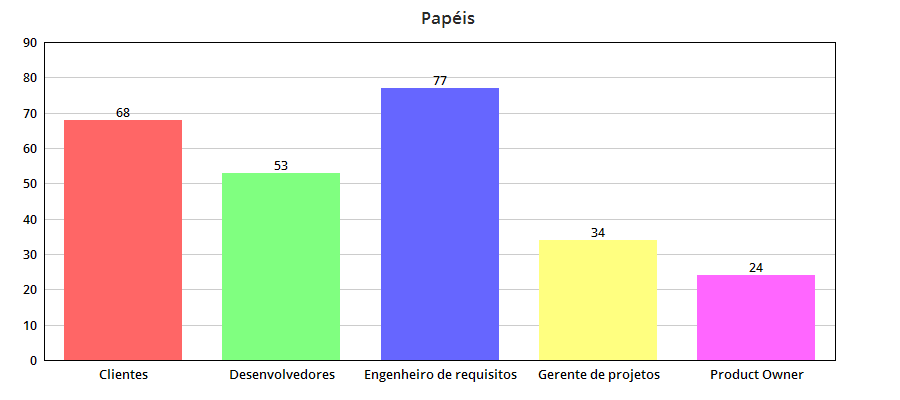
\includegraphics[scale=0.4]{figuras/grafpap.png} % altere o atributo scale para o tamanho da figura
	\end{center}
	\label{fig:grafpap}
	\legend{Fonte: Elaborado pelo autor.}
\end{figure}

\section{P2. Quais são os problemas de comunicação reportados no estudo?}

Observou-se que o maior deficit de comunicação está relacionado na fase de elicitação, já espera-se que seja uma fase crítica pois lida com a fase de indivíduos de domínios diferentes que necessitam trocar informações.
A natureza dos problemas em maior parte mostrou-se de origem humana e organizacional, podendo concluir então que uma abordagem nessas áreas poderia vir a melhorar o fluxo de comunicação.

\section{P3. Quais são os fatores de comunicação apontados no estudo?}

A partir da análise dos trabalhos selecionados foi identificado um total de 38 fatores distribuídos em 22 positivos e 16 negativos que afetam direta ou indiretamente na comunicação de requisitos no desenvolvimento de software,  Identificou-se que os fatores possuem naturezas diversas sendo bem evidentes a natureza sociocultural e organizacional, além disso a maioria dos fatores afeta em mais de um aspecto do processo de comunicação.

Os estudos selecionados evidenciaram que projetos com equipes dispersas globalmente sofrem problemas severos na comunicação. Observou-se também que o entendimento do domínio na elicitação de requisitos entre as partes envolvidas auxilia na comunicação assim como técnicas de elicitação já conhecidas. Outro fator preponderante na comunicação é a confiança entre o emissor e receptor, assim como fatores como requisitos vagos e incompletos.

Distâncias cognitivas, o tipo de linguagem, idiomas e metodologias ágeis também obtiveram uma representação considerável na pesquisa. Também é importante ressaltar que a inexistência de alguns dos fatores positivos pode acarretar em um problema na comunicação ou um pior processo no repasse de informações. Os fatores que influenciam positivamente na comunicação estão descritos na Tabela \ref{tab:fatoresP}.

%\usepackage{longtable}
\begin{longtable}{|p{5cm}|p{10cm}|}
\caption{Lista de Fatores Negativos.}

%\begin{longtable}[]
%\begin{tabular}{|p{6cm}|p{9cm}|}
\hline
\textbf{Fatores Positivos}                                                    & \textbf{Referência}                                                \\ \hline
Conhecimento do domínio                                                       & \cite{herbsleb2007global} \cite{hilbrich2017enforcing} \cite{schneider2017reframing} \cite{gates1997identification} \cite{aranda2009analyzing}  \cite{5457325},                                       \\ \hline
Uso de Vídeos/Videoconferência                                                & \cite{Oran:2017:ARC:3131151.3131166}, \cite{calazans2017software}  \cite{alnuem2012requirements} \cite{ali2016method} \cite{korkala2009distributed}
            \\ \hline
Metodologia ágil em ambientes globais                                         & \cite{knauss2014openness} \cite{noordeloos2012rup} \cite{wilks2012self} \cite{wongthongtham2006ontology} \cite{Hess2018}             \\ \hline
Documentação técnica e precisa                                                & \cite{soltani2015cross}\cite{knauss2014openness}, \cite{liskin2015artifacts} \cite{PERNSTAL201544} 
    \\ \hline
Comunicação cara a cara                                                       & \cite{wongthongtham2006ontology} \cite{Hess2018} \cite{aranda2009analyzing}
 \cite{korkala2009distributed}                                           \\ \hline
Uso de UML                                                                    & \cite{wasson2006case} \cite{diel2016communication} \cite{schneider2017reframing}, \cite{karlsson2007requirements}                   \\ \hline
Uso da linguagem nativa entre comunicadores                                   & \cite{aranda2009analyzing} \cite{6337317}             \cite{Takura19961716}                                                            \\ \hline
Interação constante                                                           & \cite{noordeloos2012rup} \cite{marnewick2011perspective} \cite{dos2013impact}  
            \\ \hline
Especificação de requisitos precisa                                          & \cite{5457325} \cite{tu2016experiment} \cite{unknown2006}
 \cite{Takura19961716}            
        \\ \hline
Comunicação entre os usuários e o engenheiro de requisitos                    &  \cite{hagelstein1988declarative} \cite{laporti2009athena}             \cite{8051365}                                                       \\     \\\hline
Contato próximo com os usuários                                               & \cite{hagelstein1988declarative} \cite{laporti2009athena}             \cite{Rauterberg1995391}                                              \\     \\\hline
Uso de sistemas de controle de versão                                         &    \cite{wasson2006case} \cite{6606709}                                \\ \hline
Analista de requisitos com proficiência em comunicação                        & \cite{sedelmaier2017can} \cite{Anwar2016726}                '            \\ \hline
Fóruns de discussão                                                           & \cite{alnuem2012requirements} \cite{8051365}                          \\ \hline
Maior transparência em documentos                                             & \cite{Oran:2017:ARC:3131151.3131166}     \cite{liskin2015artifacts}                                                     \\ \hline
Uso de Mockup e protótipos                                                    & \cite{Oran:2017:ARC:3131151.3131166} \cite{calazans2017software}        
            \\ \hline

Ferramenta de comunicação em grupos                                           &  \cite{bjarnason2017role}                                                \\ \hline
Prontidão de resposta                                                         & \cite{KIRITANI2015153}                                                    \\ \hline


Abordagem organizacional que permita fluxo aberto de mensagens                & \cite{6051643}                                                         \\ \hline





Uso de histórias do usuário                                                   & \cite{knauss2012detecting}                                            \\ \hline


Discussões contextuais em torno dos requisitos                                & \cite{stapel2009using}                                                  \\ \hline

Comunicação humana escrita com figuras, diagramas ou tabelas para sua clareza & \cite{8267930}                                                           \\ \hline


\caption{Fonte: Elaborado pelo autor}
%\end{tabular}
\label{tab:fatoresP}


\end{longtable}
\newpage

%\legend {\fontsize{10}{12}\selectfont {Fonte: Elaborado pela autor.}}
Os fatores que influenciam negativamente a comunicação estão descritos na Tabela \ref{tab:fatoresN}. 

\begin{longtable}{|p{5cm}|p{10cm}|}
%\begin{tabular}{|p{6cm}|p{9cm}|}
\caption{Fatores Negativos}

\hline
\textbf{Fatores Negativos}                                   & \textbf{Referência}                                                                                                                                                                                                                                                                                                                                                       \\ \hline

Diferenças socioculturais                                    & %\begin{tabular}[c]{@{}l@{}} 
\cite{herbsleb2007global}
\cite{wasson2006case}
\cite{diel2016communication}
\cite{alnuem2012requirements}
\cite{noordeloos2012rup}
\cite{aceituna2014model}
\cite{khan2014proposed}
\cite{Mohamad2017179}
\cite{Ghanbari201532}
\cite{5457325}\cite{aranda2009analyzing}\cite{6743519}\cite{6337317}\cite{8357767}\cite{unknown}\cite{korkala2009distributed}
%\end{tabular}                                              
\\ \hline
Distância geográfica                                         & 
\cite{wasson2006case}\cite{diel2016communication}\cite{alnuem2012requirements}\cite{noordeloos2012rup}\cite{mellhorn2017improving}\cite{calazans2017software}\cite{liskin2012improving}\cite{wongthongtham2006ontology}\cite{aceituna2014model}\cite{khan2014proposed}\cite{jeffrey1996addressing}\cite{5457325}\cite{6743519}\cite{6337317}\cite{8357767} \cite{Bjarnason2017}\cite{korkala2009distributed}

\\ \hline
Falta de confiança entre a equipe                            & 
\cite{diel2016communication}
\cite{noordeloos2012rup}\cite{xia2017personality}\cite{wu2015analysis}\cite{marnewick2011perspective}\cite{kiritani2015success}\cite{khan2014proposed}\cite{unknown}\cite{unknown2006}\cite{Anwar2016726}
            
\\ \hline
Requisitos vagos e incompletos                               & 
\cite{soltani2015cross} \cite{karlsson2007requirements}\cite{kiritani2015success}\cite{ali2016method}\cite{Jarke2011992} \cite{Ghanbari201532}                                       \\ \hline
Exclusão e distorção de informações                          &  \cite{echeverria2017influence}\cite{soltani2015cross}\cite{cois2014modern}\cite{sinha2006enabling}\cite{aceituna2014model}\cite{Tu2016}                                                                                       \\ \hline
Falta de compreensão mútua                                   &  \cite{wu2015analysis}\cite{karlsson2007requirements}\cite{khan2014proposed}\cite{unknown}\cite{Amrit:2017:EME:3084381.3084413}                                                                                                                                             \\ \hline
Diferentes idiomas falados por partes interessadas      &      \cite{pilat2011knowledge} \cite{mahmood2013software} \cite{khan2014proposed}                                                                                                                                                                                                         \\ \hline
Distâncias cognitivas (diferenças de conhecimento)           &                      \cite{mellhorn2017improving}  \cite{pilat2011knowledge}  \cite{maier2006identifying}                                                                                                                                                                                                                 \\ \hline
Frequência de comunicação baixa                              &                          \cite{diel2016communication}           \cite{marnewick2011perspective}                                                             \\ \hline
Limitação técnica no projeto                                 &       \cite{bjarnason2017role} \cite{sedelmaier2017can}                            \\ \hline
Incertezas do cliente quanto aos requisitos                  &  \cite{soltani2015cross}
\\ \hline

Incluir mais requisitos do que o especificado                &            \cite{bjarnason2011requirements}
\\ \hline


Participação inadequada dos clientes                         &             \cite{Ghanbari201532}
\\ \hline
Ambiguidade em escrita de história de usuário e casos de uso &                                                                                                                                          \cite{mahmood2013software}                                                                                                                                                                                                              \\ \hline
Falta de entendimento do canal de comunicação                &                                                                                                                                                                                                              \cite{mellhorn2017improving}                                                                                                                                        \\ \hline

\caption{Fonte: Elaborado pelo autor}

%\end{tabular}
\label{tab:fatoresN}

\end{longtable}

\newpage

 A Figura \ref{fig:graf2} ilustra a  ocorrência dos fatores positivos que apareceram quatro vezes ou mais nos estudos selecionados.



	\begin{figure}[h!] 
   	    \captionsetup{width=16cm}%Da mesma largura que a figura
		\Caption{\label{fig:graf2} Ocorrência dos fatores positivos.}
		\UFCfig{}{
			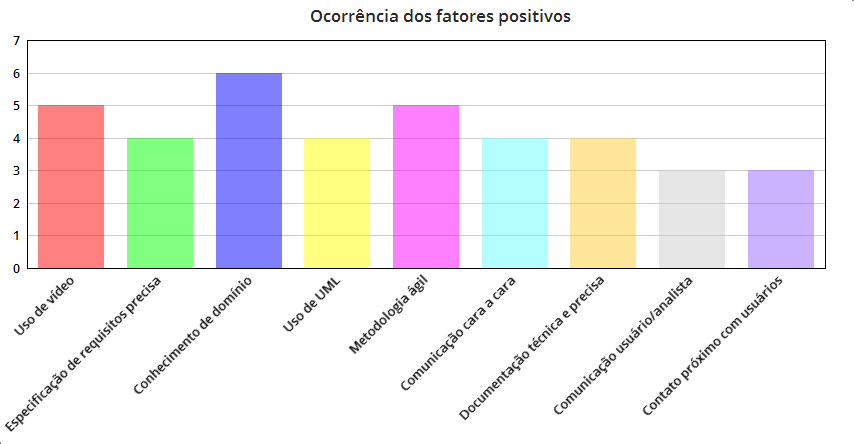
\includegraphics[width=16cm]{figuras/ChartGo.png}
		}{
			\Fonte{Fonte: Elaborado pelo autor.}
		}	
	\end{figure}
   
Na ocorrência de fatores negativos observou-se que fatores de natureza humana sobressaíram em relação aos outros. A Figura \ref{fig:ocnega}
ilustra a ocorrência de fatores negativos que surgiram quatro vezes ou mais na pesquisa. 
   

\begin{figure}[h!] 
   	    \captionsetup{width=16cm}%Da mesma largura que a figura
		\Caption{\label{fig:ocnega} Ocorrência dos fatores negativos.}
		\UFCfig{}{
			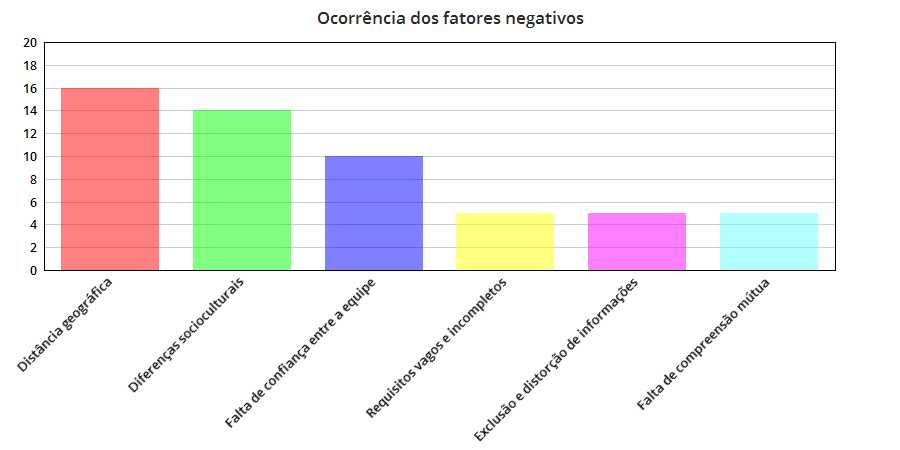
\includegraphics[width=16cm]{figuras/ocnega.png}
		}{
			\Fonte{Fonte: Elaborado pelo autor.}
		}	
	\end{figure}
   

\section{P4. Qual o impacto do fator de comunicação?}

 Foi realizado um levantamento do impacto dos fatores no processo de engenharia de requisitos considerando a escala ``grave'', ``médio'' e ``leve'', Sendo considerado grave todo e qualquer fator que acarretasse na oclusão e distorção de informações e ocorressem com maior frequência, médio fatores que causassem falhas na comunicação com uma frequência branda, e leve fatores que causassem apenas simples falhas.
 
 
 Os resultados ajudam a validar o quão a comunicação é importante na etapa de engenharia de requisitos. Por consenso foi acordado que todos os fatores afetam entre ``grave'' e ``médio'' em requisitos, visto que todos têm a possibilidade de causar distorções e falta de informações relevantes no fluxo de requisitos.
 
    Sendo descritos como graves os seguintes fatores: 
"Diferenças socioculturais", "Falta de colaboração de desenvolvedores", "Falta de confiança entre a equipe", "Distância geográfica", "Frequência de comunicação baixa", "Incertezas do cliente quanto aos requisitos" e "Requisitos Vagos e incompletos" o restante sendo classificado como de médio impacto, os resultados estão ilustrados na Figura \ref{fig:grafimpact}.


\begin{figure}[h!] %use h para forçar que a figura fique abaixo do texto
	\caption{Percentual do impacto dos fatores.}
	\begin{center}
	    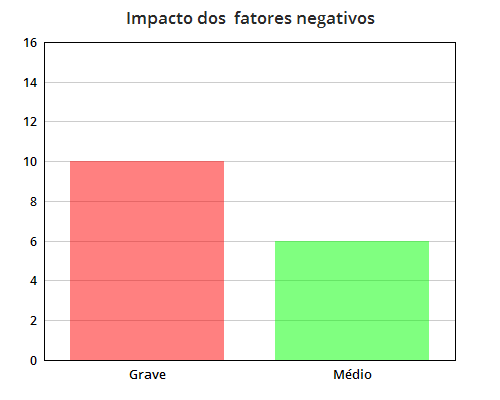
\includegraphics[scale=0.5]{figuras/impact.png} % altere o atributo scale para o tamanho da figura
	\end{center}
	\label{fig:grafimpact}
	\legend{Fonte: Elaborado pelo autor.}
\end{figure}

\section{P5. O fator interfere em qual aspecto do processo de comunicação?}

Os resultados demonstram uma maior ocorrência de fatores positivos afetando o canal de comunicação como demonstrado na Figura \ref{fig:graf}. Sendo assim, é possível inferir que os canais de comunicação bem definidos e eficientes são de grande relevância na engenharia de requisitos. 

\newpage
   \begin{figure}[h!] %use h para forçar que a figura fique abaixo do texto
    \caption{Fatores positivos no processo de comunicação.}
	\begin{center}
	    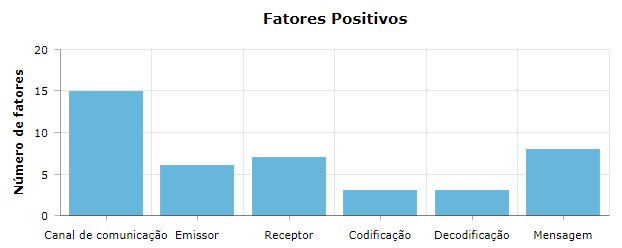
\includegraphics[scale=0.9]{figuras/graftcc} % altere o atributo scale para o tamanho da figura
	\end{center}
	\label{fig:graf}
	\legend{Fonte: Elaborado pelo autor.}
\end{figure}

Os fatores negativos ocorrem com maior frequência na emissão e recepção de dados na comunicação, com destaque também para a codificação e decodificação visto que estão estreitamente correlacionados. Este fato evidencia que o problema ocorre em repassar e receber dados e requisitos de forma correta.  

\begin{figure}[h!] %use h para forçar que a figura fique abaixo do texto

	\begin{center}
	    \caption{Fatores negativos no processo de comunicação.}
	    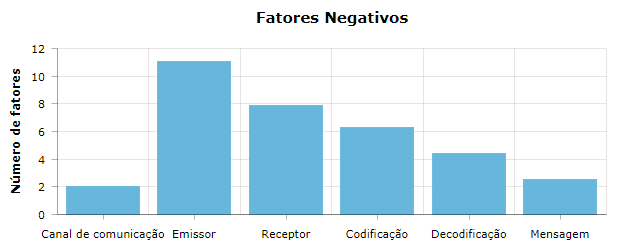
\includegraphics[scale=0.9]{figuras/graftcc1} % altere o atributo scale para o tamanho da figura
	\end{center}
	\label{fig:graft}
	\legend{Fonte: Elaborado pelo autor.}
\end{figure}

   
\section{Modelo de classificação dos fatores}

A construção do modelo foi realizada observando em qual aspecto o fator afeta no processo de comunicação, possibilitando assim obter uma classificação dos fatores regida pelo processo de comunicação, dessa forma obtém-se uma visão geral disposta em quadros que identificam os fatores positivos e negativos, podendo obter informações de quais fatores são, onde atuam e se seu impacto é benéfico ou prejudicial. 

\subsection{Fatores no canal de comunicação}

Foi identificado que os estudos levantados nessa pesquisa relatam que o canal de comunicação bem definido e técnico possui capacidade efetiva de repassar informações, Observou-se também que técnicas de elicitação atuando como canal de comunicação se tornam bastante eficazes no que propõem (ver Figura \ref{fig:quadro1}).
 
\begin{figure}[h!] %use h para forçar que a figura fique abaixo do texto
    \caption{Canal de comunicação - Fatores positivos.}
	\begin{center}
	    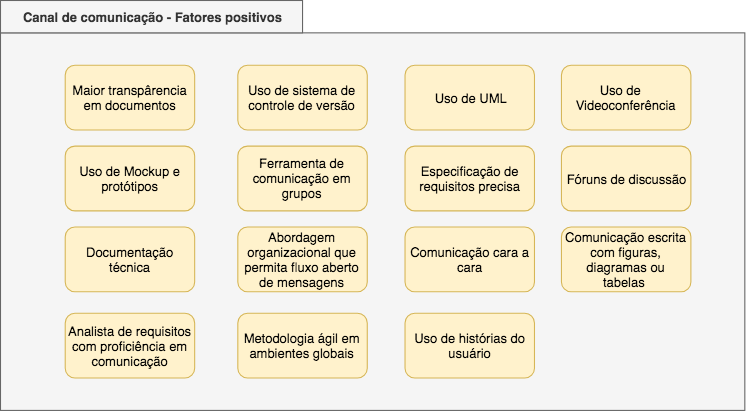
\includegraphics[scale=0.6]{figuras/quadro1} % altere o atributo scale para o tamanho da figura
	\end{center}
	\label{fig:quadro1}
	\legend{Fonte: Elaborado pelo autor.}
\end{figure}


Em contrapartida somente dois fatores negativos são relacionados ao canal de comunicação como ilustrado na Figura \ref{fig:quadro2}.
\newpage
\begin{figure}[h!] %use h para forçar que a figura fique abaixo do texto
\caption{Canal de comunicação - Fatores negativos.}
	\begin{center}
	    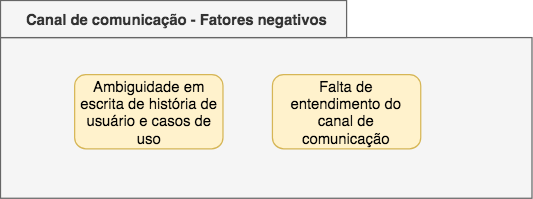
\includegraphics[scale=0.6]{figuras/quadro2} % altere o atributo scale para o tamanho da figura
	\end{center}
	\label{fig:quadro2}
	\legend{Fonte: Elaborado pelo autor}
\end{figure}

\subsection{Fatores de comunicação em emissor e receptor}

Os fatores positivos relacionados ao emissor e receptor são estritamente correlacionados, pois a emissão e recepção de uma mensagem é assíncrona, ou seja, o receptor ora pode se comportar como emissor e vice e versa, com exceção do fator "Prontidão de resposta" que diz respeito somente ao receptor (ver Figura \ref{fig:quadro3} e \ref{fig:quadroneg}).


\begin{figure}[h!] %use h para forçar que a figura fique abaixo do texto
\caption{Emissor - Fatores positivos.}
	\begin{center}
	    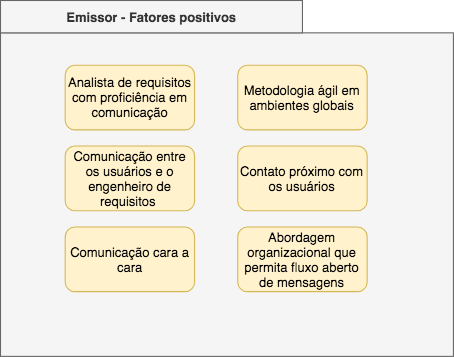
\includegraphics[scale=0.6]{figuras/quadro3} % altere o atributo scale para o tamanho da figura
	\end{center}
	\label{fig:quadro3}
	\legend{Fonte: Elaborado pelo autor.}
\end{figure}

\newpage


\begin{figure}[h!] %use h para forçar que a figura fique abaixo do texto
	\begin{center}
	
	\caption{Receptor - Fatores positivos.}
		\label{fig:quadroneg}
	    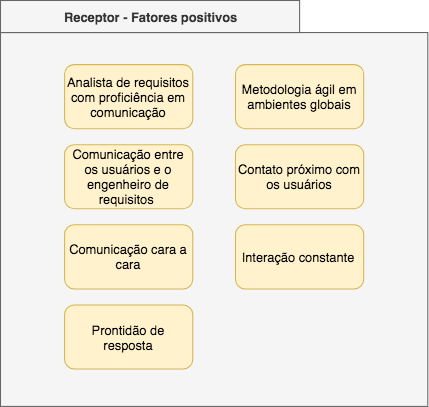
\includegraphics[scale=0.6]{figuras/quadro4} % altere o atributo scale para o tamanho da figura
	\end{center}

	\legend{Fonte: Elaborado pelo autor.}
\end{figure}

Nos fatores negativos no emissor e receptor existe uma recorrência de influência em falhas e ruídos de comunicação nesses aspectos, o que evidencia que no desenvolvimento de software é importante uma abordagem que melhore a relação emissor/receptor que ocorre em todo o processo de desenvolvimento (ver Figura \ref{fig:quadro5} e \ref{fig:quadro6}).

\begin{figure}[h!] %use h para forçar que a figura fique abaixo do texto
	\begin{center}
	    \caption{Emissor - Fatores negativos.}
	    \label{fig:quadro5}
	    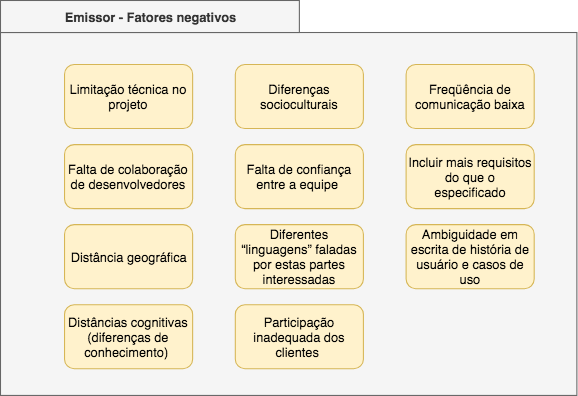
\includegraphics[scale=0.55]{figuras/quadro5} % altere o atributo scale para o tamanho da figura
	\end{center}
	
	\legend{Fonte: Elaborado pelo autor}
\end{figure}
\begin{figure}[h!] %use h para forçar que a figura fique abaixo do texto

	\begin{center}
	    \caption{Receptor - Fatores negativos.}
	    	\label{fig:quadro6}
	    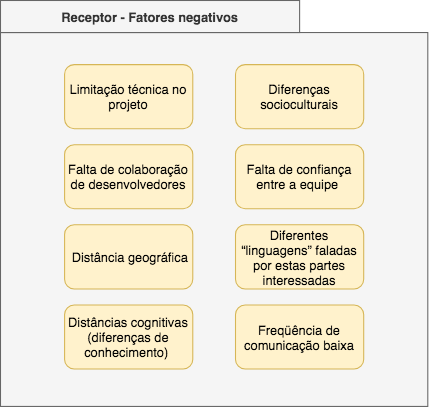
\includegraphics[scale=0.55]{figuras/quadro6} % altere o atributo scale para o tamanho da figura
	\end{center}

	\legend{Fonte: Elaborado pelo autor.}
\end{figure}

\subsection{Fatores de comunicação em codificação e decodificação}
Os fatores em codificação e decodificação assim como emissor e receptor são altamente atrelados visto que uma mensagem exige o mesmo conhecimento por parte do emissor para codifica-lá e tal qual o receptor para decodifica-lá, os mesmos se mostraram peculiares e restritos, e exclusivamente de natureza técnica organizacional e sociocultural (Ver Figura \ref{fig:quadro7}).

\begin{figure}[h!] %use h para forçar que a figura fique abaixo do texto
	\begin{center}
	    \caption{Codificação e decodificação - Fatores Positivos.}
	    \label{fig:quadro7}
	    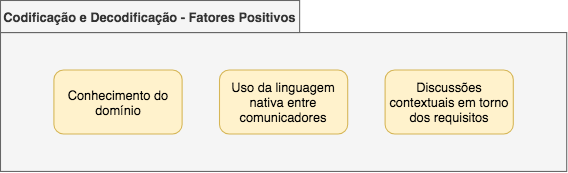
\includegraphics[scale=0.6]{figuras/quadro7} % altere o atributo scale para o tamanho da figura
	\end{center}
	
	\legend{Fonte: Elaborado pelo autor.}
\end{figure}

Para reforçar, os fatores negativos nos mesmos atuam em falhas humanas de comunicação, ex: "falta de compreensão mútua", "incerteza do cliente quanto aos requisitos" assim como falhas organizacionais (Ver Figura \ref{fig:quadro8}). 


\begin{figure}[h!] %use h para forçar que a figura fique abaixo do texto
	\begin{center}
	    \caption{Codificação e decodificação - Fatores negativos.}
	    	\label{fig:quadro8}
	    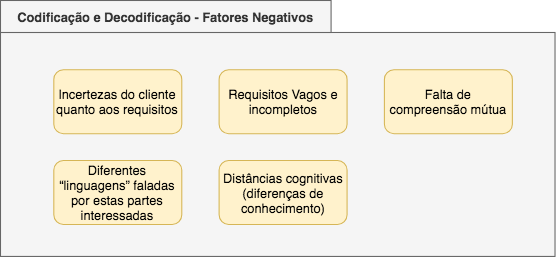
\includegraphics[scale=0.6]{figuras/quadro8} % altere o atributo scale para o tamanho da figura
	\end{center}

	\legend{Fonte: Elaborado pelo autor.}
\end{figure}

\subsection{Fatores de comunicação em mensagens}

A mensagem é relacionada com o canal de comunicação, visto que é a partir do canal que a mensagem flui, os fatores positivos em mensagem foram justamente a aplicação dos canais de comunicação já eficientes na elicitação de requisitos (Ver Figura \ref{fig:quadro9}), destacando os fatores "Maior transparência em documentos" e  "Documentação técnica" que definem uma abrangência considerável na engenharia de requisitos.


\begin{figure}[h!] %use h para forçar que a figura fique abaixo do texto
	\begin{center}
	    \caption{Mensagem - Fatores positivos.}
	    	\label{fig:quadro9}
	    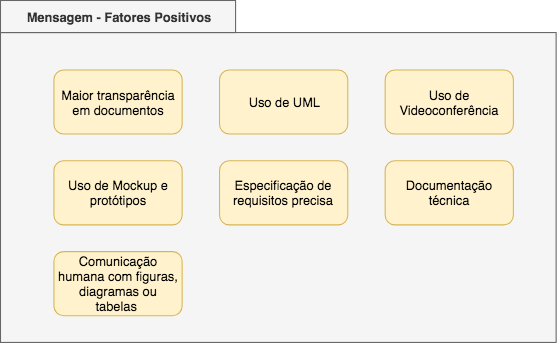
\includegraphics[scale=0.6]{figuras/quadro9} % altere o atributo scale para o tamanho da figura
	\end{center}

	\legend{Fonte: Elaborado pelo autor.}
\end{figure}

O impacto dos fatores negativos em mensagem se mostraram altamente prejudiciais, levando em conta que os mesmos dizem respeito a distorcer, excluir e diminuir a informação que deve ser repassada, algo que pode acarretar falhas graves se tratando de requisitos (ver Figura \ref{fig:quadro10}). 

\begin{figure}[h!] %use h para forçar que a figura fique abaixo do texto
	\begin{center}
	    \caption{Mensagem - Fatores negativos.}
	    	\label{fig:quadro10}
	    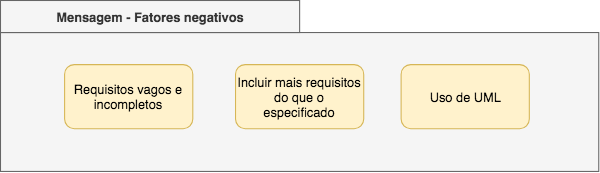
\includegraphics[scale=0.6]{figuras/quadro10} % altere o atributo scale para o tamanho da figura
	\end{center}

	\legend{Fonte: Elaborado pelo autor.}
\end{figure}

%{tabular}{|p{2.5cm}|p{2.2cm}|p{2.0cm}|p{2.0cm}|p{2.0cm}| }

A próxima seção apresenta a conclusão e propostas de trabalhos futuros. 

\newpage















   


	\chapter{CONCLUSÃO E TRABALHOS FUTUROS}
\label{chap:conclusoes-e-trabalhos-futuros}



A fase de engenharia de requisitos é a mais crítica uma vez que uma grande proporção de problemas no desenvolvimento são derivados de problemas com os requisitos. Um dos aspectos no processo de engenharia de requisitos essenciais para sua eficácia é a comunicação. Esta contribui para que as informações fluam sem conflitos em toda a extensão do projeto. Portanto, garantir uma boa comunicação proporciona flexibilidade e rapidez no processo.

Existem fatores que influenciam, positivamente e negativamente, a comunicação de requisitos em diferentes etapas do processo. Sendo assim, o estudo de fatores que impactam a comunicação de requisitos é de fundamental importância para obter melhores resultados no desenvolvimento de software. Nesse contexto, proporcionar melhorias na comunicação em todo o processo é uma constante prioridade das empresas que prezam por processos de boa qualidade.

Este trabalho teve como objetivo identificar fatores que interferem na comunicação de requisitos ao longo do desenvolvimento de software, Para alcançar tal meta, uma revisão sistemática da literatura foi realizada. A revisão retornou 860 trabalhos dos quais 94 foram aceitos para extração.

Sendo assim, este trabalho possibilitou responder as seguintes perguntas de pesquisa:

\textbf{P1: Quais são os stakeholders envolvidos?} observou-se um deficit de comunicação nos papéis de clientes, engenheiro de requisitos e desenvolvedores.

\textbf{P2: Quais são os fatores de comunicação apontados no estudo?} este trabalho identificou um total de 38 fatores distribuídos em positivos e negativos.

\textbf{P3: Quais são os problemas de comunicação reportados no estudo?}, foi identificado 16 fatores de comunicações negativos que ocasionam problemas na comunicação. 

\textbf{P4: Qual o impacto do fator de comunicação?} a gravidade dos fatores se mostrou critica devido ao fato de influenciarem na distorção e oclusão de informações ameaçando assim a qualidade do projeto. Os fatores foram classificados como grave e médio, tendo uma distribuição de 60,64\%  e 39,36\% respectivamente.

\textbf{P5: O fator interfere em qual aspecto do processo de comunicação} observou-se que fatores positivos geralmente estão relacionados a canais de comunicação eficientes, e negativos estão relacionados a conexão emissor/receptor.

A análise mostrou também que a ocorrência dos fatores em mais de um trabalho contribuindo para a qualidade dos dados obtidos. O trabalho contribui de maneira que evidencia a existência das questões de comunicação no desenvolvimento de software, identificando fatores e a natureza de suas origens assim como a atuação e o impacto dos mesmos no processo de comunicação.

Como trabalhos futuros, sugere-se um estudo detalhado sobre os fatores identificados e sobre o modelo de classificação dos fatores assim possíveis trabalhos futuros podem ser:

\begin{itemize}
    \item Validar o modelo de classificação deste estudo por profissionais de desenvolvimento de software.
    \item Investigar formas de mitigação das falhas humanas e organizacionais de comunicação.
    \item Validar o grau em que os fatores positivos descritos realmente contribuem no repasse de informações de requisitos.
    \item Avaliar a qualidade dos estudos selecionados neste trabalho.

\end{itemize}


 \newpage 

	
	%Elementos pós-textuais	
	\bibliography{3-pos-textuais/referencias}
%	\imprimirglossario	
	%\imprimirapendices
		% Adicione aqui os apendices do seu trabalho
	%	\apendice{Exemplo de apêndice}
\label{ap:A}

Um apêndice é um documento elaborado pelo autor, diferentemente do anexo. Geralmente, se coloca como apêndice, questionários, códigos de programação, tabelas que tomariam muito espaço no meio do trabalho. Artigos, resumos ou qualquer publicação relacionada ao trabalho podem ser utilizados como apêndice.
	%	\apendice{Questionário utilizado para...}
\label{ap:B}

\begin{questao}
	\item Esta é a primeira questão com alguns itens:
		\begin{enumerate}
			\item Este é o primeiro item
			\item Segundo item
		\end{enumerate}
	\item Esta é a segunda questão:
		\begin{enumerate}
			\item Este é o primeiro item
			\item Segundo item
		\end{enumerate}
	\item Lorem ipsum dolor sit amet, consectetur adipiscing elit. Nunc dictum sed tortor nec viverra. consectetur adipiscing elit. Nunc dictum sed tortor nec viverra.
		\begin{enumerate}
			\item consectetur
			\item adipiscing
			\item Nunc
			\item dictum
		\end{enumerate}
\end{questao}

	%	\apendice{Códigos-fontes utilizados para...}
\label{ap:C}

\lstinputlisting[language=C++,caption={Hello World em C++}]{figuras/main.cpp}


\begin{lstlisting}[language=Java,caption={Hello World em Java}]
public class HelloWorld {
	public static void main(String[] args) {
		System.out.println("Hello World!");
	}
}
\end{lstlisting}


	%	\apendice{\textit{IEEE CEFC 2016}}
\label{ap:D}

\textit{Digest} submetido ao \textit{The 17th Biennial Conference on Eletromagnetic Field Computation, Miami FL - NOV 13-16, 2016, USA}.

%Código fonte para inserir um arquivo em PDF
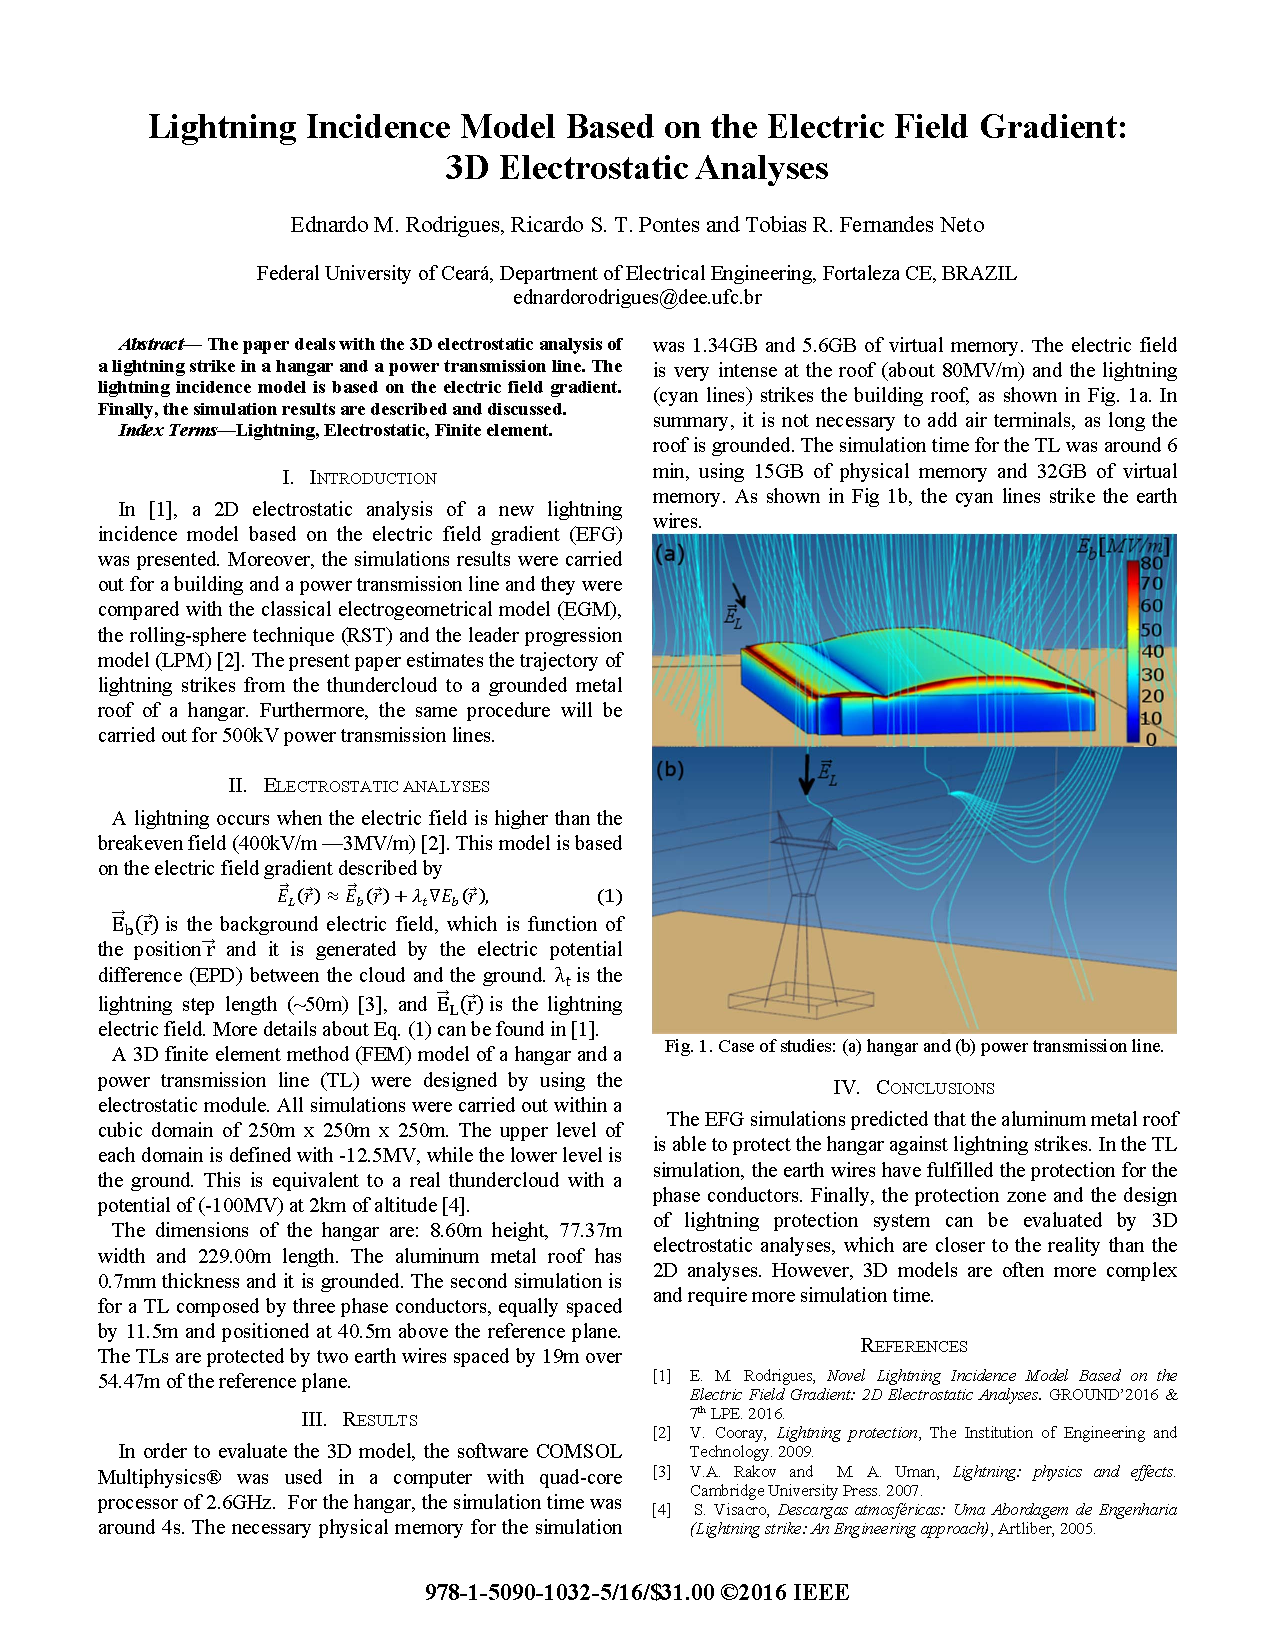
\includepdf[pages={-}]{3-pos-textuais/apendices/PID4416093.pdf}
	%\imprimiranexos
		% Adicione aqui os anexos do seu trabalho
		%\anexo{Exemplo de um anexo}
\label{an:ex_anexo_a}

Um anexo é um documento que não foi elaborado pelo autor, ou seja, o autor apenas anexa. Anexos podem ser tabelas, mapas, diagramas, \textit{datasheets}, manuais e etc. 




	%	\anexo{Exemplo de um anexo em PDF}
\label{an:ex_anexo_b}

O autor pode anexar um \gls{PDF}, traduzido como formato portátil de documento. Veja o código fonte utilizado para anexar o arquivo ``Sikasil.pdf'' que foi colocado dentro da pasta ``anexos'' que por sua vez está dentro da pasta ``elementos-pos-textuais''. Tenha muita atenção na hora de especificar o local do arquivo. Recomenda-se não utilizar caracteres especiais para nomear pastas e, principalmente, arquivos. 

Pode-se fazer uma descrição sucinta do arquivo anexado.

%Comando para incluir um arquivo em PDF:
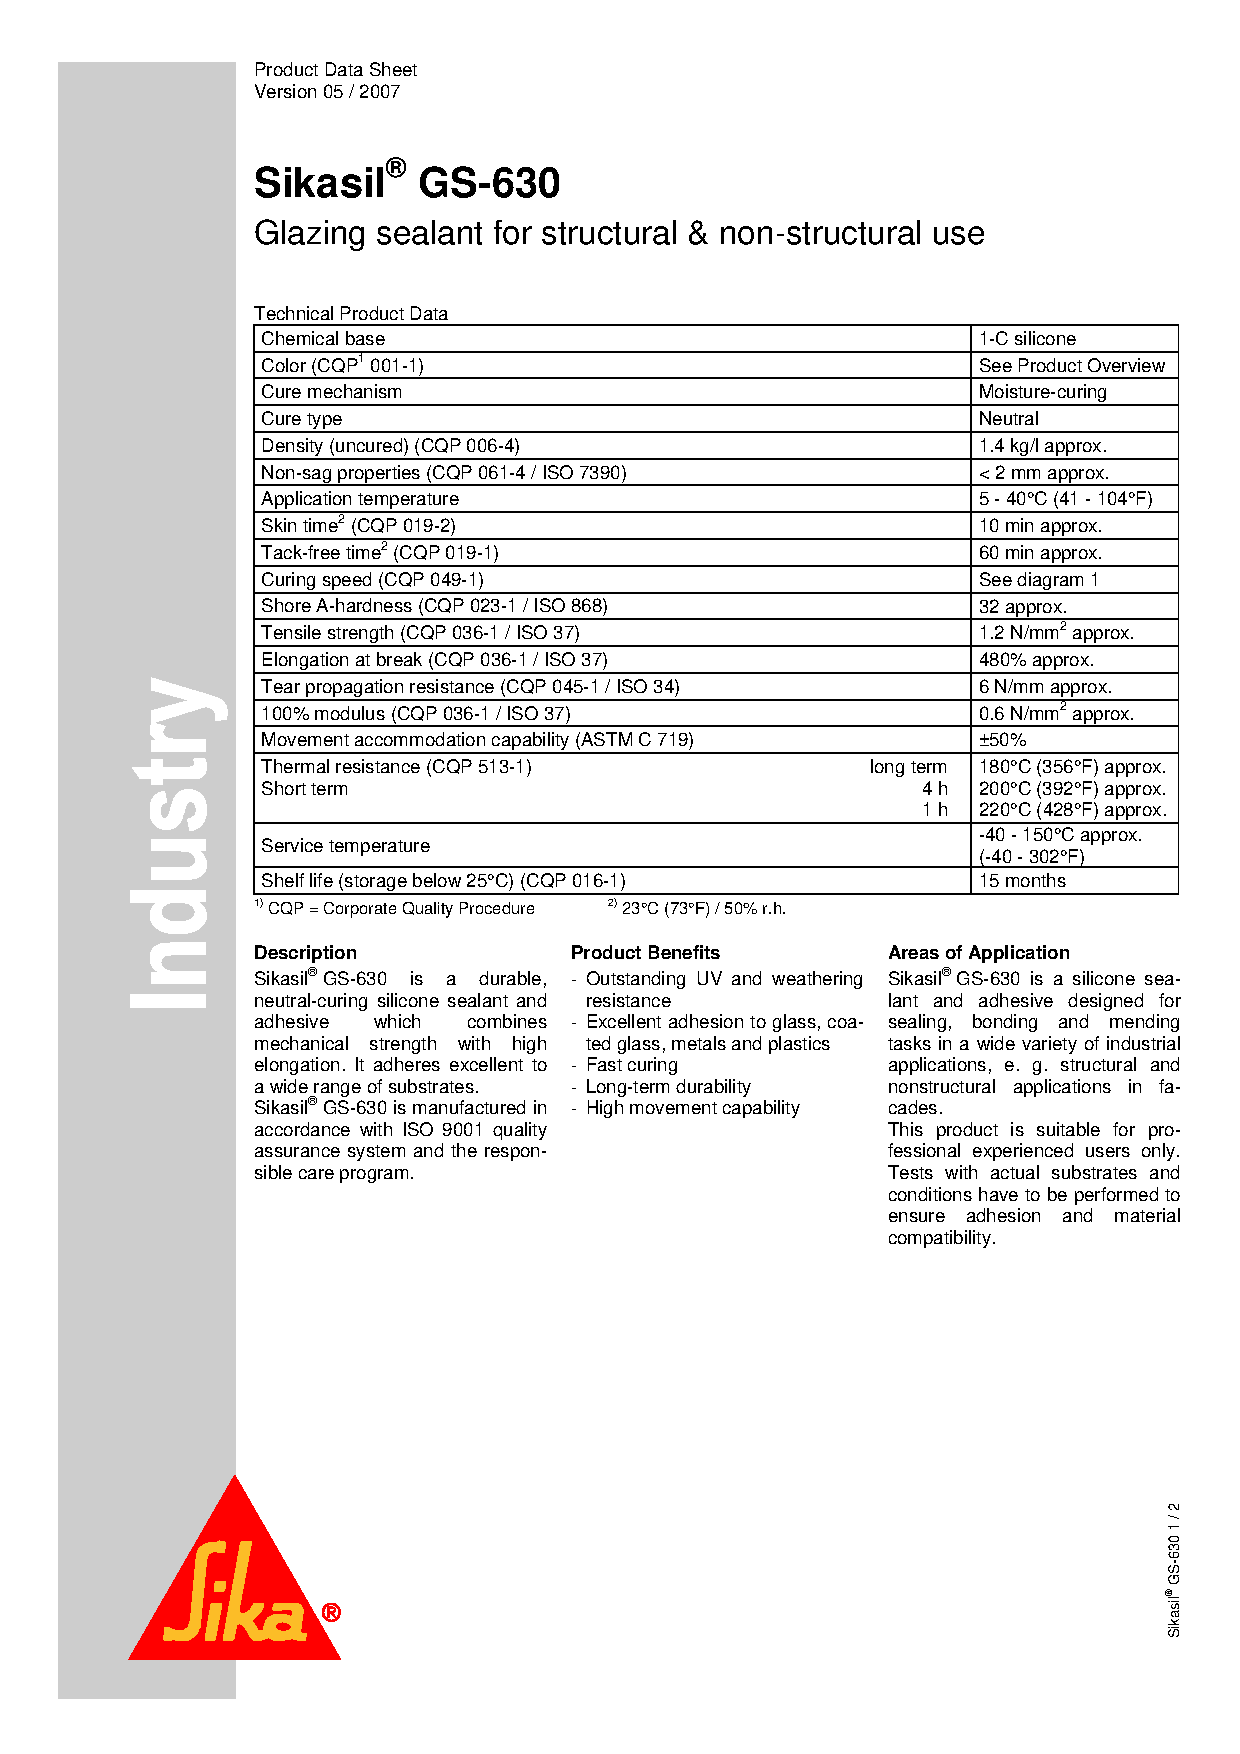
\includepdf[pages={-}]{3-pos-textuais/anexos/Sikasil.pdf}

		
	%\imprimirindice

\end{document}